\documentclass[12pt,a4paper]{article}
\usepackage[utf8]{inputenc}
\usepackage[provide=*]{babel}
\babelprovide[import=de, main]{de}
\usepackage[T1]{fontenc}
\usepackage{geometry}
\geometry{a4paper, left=2.5cm, right=2.5cm, top=3cm, bottom=3cm}
\usepackage{graphicx}
\usepackage{hyperref}
\usepackage{tikz}
\usetikzlibrary{shapes.geometric, arrows.meta, positioning, fit, backgrounds}
\usepackage{enumitem}
\usepackage{tabularx}
\usepackage{xcolor}
\usepackage{amsmath}
\usepackage{float}


\title{\textbf{Arbeitsexposé}\\KI-gestützte 3D-Rekonstruktion linearer Infrastruktur: Evaluierung einer Docker-basierten Scan-to-BIM Pipeline mittels SAM 3 und Gaussian Splatting}
\author{Bachelor- und Projektarbeit}
\date{\today}

\begin{document}

\maketitle

\section{Einleitung und Forschungsfrage}
Die präzise Erfassung schwer zu modellierender, extrem dünner Objekte (wie Stromerdkabel in Baugräben) stellt für klassische photogrammetrische Verfahren (SfM) eine große Herausforderung dar. Ziel dieser Arbeit ist die Entwicklung und Evaluierung eines "Scan-to-BIM"-Workflows, der die Vorzüge der 2D-KI-Segmentierung (Segment Anything Model 3) mit modernsten 3D-Rekonstruktionsmethoden (3D Gaussian Splatting via SuGaR) verbindet.

Wie aktuelle Forschungen belegen, erzeugen 3D Gaussian Splatting Algorithmen durch mathematische Wahrscheinlichkeitsfunktionen hochgradig detailreiche, fotorealistische Visualisierungen bei geringer Rechenlast. Sie werden zunehmend im Ingenieurwesen und zur Generierung von Orthofotos (z.B. Integration in ArcGIS Pro) eingesetzt. Jedoch fehlt 3DGS-Modellen die inhärente Georeferenzierung.
Die zentrale Forschungsfrage lautet daher: \textit{Lässt sich die 3D-Rekonstruktion linearer Infrastruktur durch eine vorgelagerte 2D-Segmentierung und ein objektspezifisches 3DGS-Training (Segment-then-Splat) so optimieren und georeferenzieren, dass strenge ingenieurstechnische Toleranzen eingehalten werden?}

\section{Praxisbezug und Erfolgskriterien}
Die Pipeline wird direkt für den Anwendungsfall der TenneT (Übertragungsnetzbetreiber) konzipiert.
\begin{itemize}
    \item \textbf{Geometrische Toleranz:} Eine Abweichung von maximal $\pm$ 10\,cm in Lage und Höhe gegenüber der realen Kabeltrasse.
    \item \textbf{Georeferenzierung \& GIS-Integration:} Das finale 3D-Modell muss präzise in einem UTM-Koordinatensystem vorliegen, um den direkten Import in Geoinformationssysteme (z.B. ArcGIS Pro) zu gewährleisten.
    \item \textbf{Wirtschaftliche Evaluierung:} Eine Kostengegenüberstellung des Drohnen- und Serverrechenaufwands im Vergleich zur klassischen, terrestrischen Vermessung.
\end{itemize}

\section{Methodik und Architektur (Workflow v3)}
Der Ansatz basiert auf einer klaren Trennung von 2D-Bildverarbeitung und 3D-Meshing.

\subsection{Software-Repositories}
\begin{itemize}
    \item \textbf{SAM 3 (Meta):} Zuständig für Concept-Prompting und Video-Tracking.
    \item \textbf{COLMAP:} Generierung der Kameraposen auf Basis der \textit{unmaskierten} Originalbilder. Die Pipeline nutzt ausschließlich das schnelle \textit{Structure from Motion} (SfM) von COLMAP. Die rechenintensive dichte Rekonstruktion (MVS) wird vollständig übersprungen.
    \item \textbf{Segment-then-Splat (STS):} Übernimmt das objektspezifische 3DGS-Training (Lu et al., NeurIPS 2025). STS teilt die initialen COLMAP-Gaussians anhand der SAM 3 Masken in objektspezifische Sets auf und trainiert diese mit einem dedizierten Object-specific Loss ($\mathcal{L}_{obj}$), ohne die Ground-Truth-Bilder zu manipulieren. Das Ergebnis ist ein vollständiges 3DGS-Modell, in dem jeder Gaussian eine Object-ID trägt. SAM 3 ersetzt hierbei das intern vorgesehene AutoSeg-SAM2.
    \item \textbf{SuGaR:} Surface extraction with Gaussian Splatting. SuGaR übernimmt einen 3DGS-Checkpoint, richtet die Gaussians mittels geometrischer Regularisierung (insbesondere Depth-Normal Consistency) an der Oberfläche aus und extrahiert über Poisson Surface Reconstruction ein Mesh. Für objektspezifische Eingaben wird SuGaR um maskenkonsistente RGB-, Normalen- und Texturverluste erweitert, damit die Bildsupervision dieselbe semantische Objektdefinition wie STS verwendet.
    \item \textbf{DGtal:} Open-Source Geometrie-Bibliothek zur finalen Centerline-Extraktion. Sie wandelt die Oberfläche des Kabel-Sub-Meshes in eine räumliche 1D-Kurve (Centerline bzw. Scheitelachse mit lokalen Koordinaten) um.
\end{itemize}

\subsection{Pipeline-Struktur: Temporale Konsistenz vs. SAHI}
Für die Erkennung extrem dünner Kabel in hochauflösenden 4K-Bildern bietet sich theoretisch \textit{Slicing Aided Hyper Inference} (SAHI) an. SAHI zerschneidet das Bild in kleinere Teilbereiche (Patches), wodurch verhindert wird, dass dünne Kabel beim Downscaling auf die native Modellauflösung von SAM 3 "verschluckt" werden.

Dennoch wurde der primäre Fokus für diese Pipeline bewusst auf den \textbf{SAM 3 Video Predictor} gelegt. Der methodische Nachteil von SAHI ist die fehlende temporale Konsistenz: Da SAHI jedes Einzelbild isoliert betrachtet, "flackern" die erzeugten Masken von Frame zu Frame, wenn sich Lichteinfall oder Blickwinkel leicht ändern. 3D Gaussian Splatting erfordert jedoch zwingend formstabile, konsistente Masken über alle Kameraperspektiven hinweg, da sonst fehlerhafte Artefakte in den 3D-Raum projiziert werden. Der SAM 3 Video Predictor löst dieses Problem durch ein Memory-Modul, welches die Kabel-Pixel über die Zeit hinweg verfolgt und dadurch flackerfreie, temporär konsistente Masken liefert. SAHI dient in dieser Pipeline lediglich als Fallback-Route für spezifische Bildausschnitte, in denen das temporale Tracking abreißen sollte.


\section{Docker-Infrastruktur und Orchestrierung}
Ein Kernproblem moderner KI-Pipelines sind tiefgreifende Versionskonflikte zwischen den benötigten Nvidia-Grafikkartentreibern (CUDA). Dieses Problem wird durch eine \texttt{docker-compose} Architektur vollständig gelöst. Die Pipeline isoliert die Anwendungen in voneinander getrennte Container, während alle erzeugten Daten über \textbf{Docker Bind Mounts (Volumes)} zentral und persistent auf dem Host-System (Windows/Linux) gespeichert werden.

Um die Automatisierung zu maximieren, wird die Pipeline über ein zentrales Master-Skript (\textit{One-Click-Orchestration}) gesteuert. Dieses Skript stößt die Container sequenziell an, muss jedoch für manuelle Arbeitsschritte pausieren. 

\textbf{Autopilot-Modus für unterbrechungsfreie Verarbeitung:}\\
Um den wissenschaftlichen Workflow anwenderfreundlich zu gestalten und manuelle Interaktionen auf ein Minimum zu reduzieren, wurde ein optionaler **Autopilot-Modus** in die Orchestrierungskonfiguration integriert. Direkt nach der Eingabe des Semantik-Prompts (z.\,B. \texttt{"cable"}) kann dieser aktiviert werden. 
*   **Wirkungsweise:** Alle nachgelagerten Parameterentscheidungen werden vollautomatisch mit vordefinierten, wissenschaftlich erprobten Standardwerten belegt. 
*   **Automatisierte Parameter:** Das FFMPEG-Pre-Processing erzeugt im aktuellen Projektarbeitsstandard ein komprimiertes Arbeitsvideo mit $1280 \times 720$ Pixeln bei $5$\,FPS, CRF $18$ und dem x264-Preset \texttt{medium}. Das STS-Training verwendet standardmäßig $7000$ Gesamtiterationen: $5000$ Iterationen fuer die Objekt-/Maskenphase und anschliessend $2000$ Iterationen fuer alle konfigurierten Objekte. Die Stage-2-Angabe ist dabei ein Curriculum-Fenster innerhalb der Gesamtzahl und kein zusaetzlicher Block nach dem Gesamttraining.
*   **Anwendervorteil:** Bis auf den zwingenden physikalischen Messschritt (Breakpoint für das GCP-Point-Picking in CloudCompare) ist kein Benutzereingriff mehr erforderlich. Die Pipeline steuert alle fünf Microservices automatisiert an, führt den neuen Teilmodell-Wechsler (Best-Model-Resolver) selbständig aus und exportiert die georeferenzierten GIS-Daten fix und fertig in das Zielverzeichnis.

Es kommen fünf dedizierte Container zum Einsatz:
\begin{itemize}
    \item \textbf{Container A (Vorverarbeitung):} Beinhaltet PyTorch 2.x und SAM 3. Benötigt das Nvidia Container Toolkit (CUDA >= 12.6).
    \item \textbf{Container B (SfM):} Ein offizielles NVIDIA-Image für COLMAP (CUDA 11.8 oder 12.1). \textit{Nach Ausführung dieses Containers pausiert das Master-Skript automatisch (Breakpoint). Der Nutzer öffnet CloudCompare auf dem Host-System, pickt die GCPs und speichert die Transformationsmatrix. Anschließend wird das Skript mit ``Enter'' fortgesetzt.}
    \item \textbf{Container C (Object-specific 3DGS):} Beinhaltet Segment-then-Splat (STS). Empfängt die SAM 3 Masken und die COLMAP-Kameraposen und führt das objektspezifische 3DGS-Training mit dem nativen Object-specific Loss ($\mathcal{L}_{obj}$) durch. Benötigt CUDA 12.1 (PyTorch 2.3.1). SAM 3 ersetzt hierbei das intern vorgesehene AutoSeg-SAM2 als Masken-Frontend.
    \item \textbf{Zwischenschritt 3.5 (Kabel-Isolierung \& Qualitätsfilterung):} Das Skript \texttt{filter\_cable\_pc.py} erzeugt zusätzlich zur unveränderten Full-Scene-Punktwolke die echt gefilterte Objektwolke \texttt{point\_cloud\_filtered.ply}. Es selektiert die konfigurierte Ziel-Objekt-ID (im aktuellen Versuchsdatensatz \texttt{obj\_id\_m == 0}) und kann Opazitäts- sowie Farbschwellen anwenden. Eine zweite Kopie, \texttt{point\_cloud\_filtered\_opacity999999.ply}, übernimmt dieselben verbliebenen Datensätze und setzt ihre Opazitätslogits für den geometrieorientierten, maskenkonsistenten SuGaR-Eingang einheitlich auf \(\alpha=0{,}999999\). Diese Überschreibung ist eine Initialisierungspolitik und keine physikalische Aussage über die Transparenz des Objekts. Die getrennte Ablage verhindert, dass ein Objekt-Checkpoint versehentlich als unmaskierte Full-Scene-SuGaR-Baseline dient.
    \item \textbf{Container D (Meshing):} Beinhaltet SuGaR. Für die Full-Scene-Baseline wird der unveränderte STS-Checkpoint verwendet; für die Objektrekonstruktion wird eine private Kopie der gefilterten Punktwolke mit maskenkonsistenter SuGaR-Optimierung verarbeitet. Danach folgen Poisson-Mesh-Extraktion, maskiertes UV-Textur-Baking und ein Multi-View-Konsens-Crop. Wegen tiefer Abhängigkeiten zum \texttt{diff-gaussian-rasterization} Modul wird hier strikt CUDA 11.8 erzwungen. Das intern geforderte Conda-Environment wird systemweit über eine Anpassung der \texttt{ENV PATH} Variable im Dockerfile nativ zugänglich gemacht.
    \item \textbf{Container E (Post-Processing):} Ein reiner \textbf{CPU-Container} (ohne GPU/CUDA-Abhängigkeit). Beinhaltet die C++ Bibliothek DGtal sowie die GDAL-Tools (\texttt{ogr2ogr}). Durch die Auslagerung dieser CPU-basierten Nachbearbeitung in einen eigenen Microservice bleibt die Architektur extrem leichtgewichtig, da keine massiven Nvidia-Images geladen werden müssen.
\end{itemize}

\section{Risikomanagement und Datenhandling}
Mehrere kritische Punkte und prozessuale Hürden erfordern besondere Aufmerksamkeit:
\begin{enumerate}
    \item \textbf{Photogrammetrischer Aufnahmestandard zur Qualitätssicherung und Vermeidung von Sub-Modellen:} \\
          Ein zentraler Erfolgsfaktor der Rekonstruktion linearer Bauteile ist die Akquisition des primären Fotomaterials. Um eine fehlerhafte Zerteilung der Punktwolke durch COLMAP in unvollständige Sub-Modelle (Splits) gänzlich zu verhindern, müssen strenge photogrammetrische Standards eingehalten werden:
          \begin{itemize}[noitemsep]
              \item \textbf{Verriegelung der inneren Orientierung (Konstante Kameraparameter):} Jede Änderung der Brennweite während der Aufnahme destabilisiert die Ausgleichungsrechnung fundamental. Der Autofokus der Kamera bzw. Drohnensensorik muss verpflichtend deaktiviert sein (Einstellung auf manuellen Fokus unendlich bzw. feste hyperfokale Distanz). Ebenso ist eine automatische Belichtung (Auto-Exposure) und ein automatischer Weißabgleich zu unterbinden, um photometrische Fehlzuordnungen der SIFT-Deskriptoren zu vermeiden.
              \item \textbf{Geometrische Überdeckung und Bildwinkel:} Die Aufnahmen müssen eine Längsüberdeckung von mindestens $80\,\%$ und eine Querüberdeckung von mindestens $60\,\%$ aufweisen. Bei linearen Objekten müssen dichte Nadir-Aufnahmen ($90^\circ$ orthogonal nach unten) planmäßig durch leicht geneigte Oblique-Aufnahmen ($15^\circ$ bis $30^\circ$ Neigungswinkel) ergänzt werden. Dies bricht die koplanare Entartung der Sichtstrahlen auf und ermöglicht dem Bündelausgleich eine saubere Rekonstruktion zylindrischer Geometrien.
              \item \textbf{Einbringung von Anker-Geometrien im Alphanumerischen Raum (Anchor Features):} Extrem glatte, einfarbige Objekte (wie das nackte Erdkabel oder Kunststoffflaschen) besitzen keine SIFT-merkmalsfähige Textur, wodurch der photogrammetrische Strahlenschnitt kollabiert. Zur physikalischen Konditionierung der Szene müssen kontrastreiche, hochfrequente Muster-Strukturen („Anker-Objekte“ wie gemusterte Markierungsmatten, beschriebene Zeitungsseiten oder künstliche codierte ArUco-Markerboards) im unmittelbaren Nahbereich um das Objekt ausgelegt werden. Diese Anker erzeugen tausende fehlerfreie Feature-Matches, an welchen COLMAP die Kameras stabil orientieren kann, während das eigentliche Zielobjekt später durch die semantische 2D-Segmentierung (SAM 3.1) sauber herausgelöst wird.
          \end{itemize}
    \item \textbf{Speichermanagement:} Drohnenvideos in 4K bei 60 FPS erzeugen massive Datenmengen. Das Konzept sieht vor, dass diese temporär im nativen Linux-Dateisystem liegen und nach der 6 FPS Extraktion gelöscht werden, um I/O-Engpässe unter WSL2 zu vermeiden.
    \item \textbf{SAM 3 Tracking-Stabilität (VRAM) und Modellkonsistenz:} \\
          In der praktischen Ausführung zeigte sich ein nichtlinear wachsender VRAM-Bedarf im \texttt{propagate\_in\_video}-Pfad (insb. während \texttt{F.interpolate} in der Output-Erzeugung). Dadurch trat ein \texttt{CUDA out of memory} nicht deterministisch auf (z. B. um Frame 45, bei anderen Läufen früher oder später), obwohl dieselbe Eingabe verwendet wurde. Ursache ist die Kombination aus langem Sequenzgedächtnis (Memory-Modul), fragmentiertem Allocator-Zustand und voller HD-Auflösung über viele Frames. \\
          Als technische Gegenmaßnahme wurde die Propagation auf feste Zeitfenster (Chunking) umgestellt: Jeder Lauf verarbeitet nur ein Segment mit \texttt{start\_frame\_index} und \texttt{max\_frame\_num\_to\_track}; die Masken werden unmittelbar pro Frame persistiert, statt alle Outputs bis zum Ende im RAM/VRAM vorzuhalten. Zusammen mit Offloading-Flags (Video/State auf CPU) stabilisiert dies die Pipeline auf 16-GB-Karten. \\
          Ein zweiter, davon getrennter Befund ist die \textbf{Gewichts-/Architektur-Konsistenz}: Trotz stabilem Lauf können aufgrund von \texttt{Missing keys}/\texttt{Unexpected keys} beim Laden des SAM-Checkpoints formal gültige, aber inhaltlich leere Masken entstehen. Daher wird als Quality-Gate vor Übergabe an STS verbindlich geprüft: (i) Anteil nichtleerer Masken, (ii) temporale Kontinuität über benachbarte Frames, (iii) Sichtprüfung an Stichproben. Nur bei erfüllten Kriterien werden Masken in Container C übernommen.
        \item \textcolor{blue}{\textbf{[GELÖST: SAM 3.1 Video-Tracking stabilisiert, Stand 06/2026]}} \\
            Die anfängliche Instabilität des SAM 3.1 Video-Pfades konnte durch drei gezielte Maßnahmen gelöst werden, was eine unterbrechungsfreie Voll-Propagation über alle 100 Frames auf einer 16-GB-GPU ermöglichte:
            (i) \textbf{VRAM-Limitierung durch sequenzielles Vision-Language-Matching}: Die Aktivierung von \texttt{batched\_grounding\_batch\_size = 1} (anstelle von standardmäßigem Batching nach Text-Prompts) reduzierte den VRAM-Verbrauch von über 12\,GB auf unter 5\,GB, wodurch jegliche \texttt{CUDA out of memory}-Fehler verhindert wurden. Zusätzlich wurde die PyTorch-Compilation via \texttt{TORCH\_COMPILE\_DISABLE=1} deaktiviert, um massive RAM/VRAM-Spitzen vorzubeugen.
            (ii) \textbf{Behebung des Shape-Assertions-Fehlers}: Der zuvor auftretende Fehler \texttt{AssertionError: pos\_pred\_mask.shape[0] == 1} bei der Chunk-Verarbeitung wurde durch Rückkehr zum globalen Video-Inferenz-Modus unter Verwendung der Standard-Konditionierungsparameter (\texttt{max\_cond\_frames\_in\_attn} unlimitiert) gelöst.
            (iii) \textbf{Datensatz-Kompatibilität bei der Masken-Persistierung}: SAM 3.1 Multiplex liefert den Vorhersage-Stream nicht in Form geschachtelter Dictionaries wie reguläre SAM-Modelle, sondern im Multiplex-spezifischen Format, d.\,h. als Dictionary mit den Hauptschlüsseln \texttt{out\_obj\_ids} und \texttt{out\_binary\_masks}. Ein angepasster Masken-Parser extrahiert nun die Binärmasken direkt über \texttt{out\_binary\_masks[idx]}.
            Durch diese Korrekturen konnte die Inferenz bei ca. 3,1\,it/s vollständig stabilisiert werden und liefert mit dem Text-Prompt \texttt{"cable"} reproduzierbar \textbf{33 nicht-leere Masken} über den 100 Frames großen Testdatensatz hinweg. \\
            \textbf{Einfache Erklärung (für Laien/Nicht-Techniker verständlich):} \\
            Zuvor brach das System beim Versuch, das Kabel im Video automatisch zu verfolgen, ständig ab oder fand schlichtweg gar nichts. Das lag an drei anschaulichen Problemen:
            \begin{itemize}
                \item \textit{Die Speicher-Überlastung (VRAM-Absturz):} Das Programm wollte alle KI-Bildanalysen für die Text-Prompts gleichzeitig im Grafikspeicher lösen. Das ist so, als ob man versucht, 10 dicke Bücher gleichzeitig auf einmal aufzuschlagen und querzulesen -- das Gehirn (die GPU) ist überfordert. Indem wir dem System befehlen, die Sätze brav nacheinander zu verarbeiten (\texttt{Batch-Größe = 1}) und das zeitaufwendige „Vorab-Auswendiglernen“ ausschalten (\texttt{Kompilierung aus}), liest die GPU das Video nun stressfrei Bild für Bild. Der Speicherbedarf sank von über 12\,GB auf gemütliche 4,5\,GB.
                \item \textit{Die Denkblockade (Der AssertionError):} Um Speicher zu sparen, hatten wir das Video anfangs in kurze 8-Bild-Häppchen zerlegt. Die KI kam bei der Übergabe der Häppchen jedoch völlig durcheinander, verlor den Faden und behauptete stur, die Teile würden logisch nicht mehr zusammenpassen. Wir lassen das Video nun einfach elegant am Stück durchlaufen und überlassen der KI die vollautomatische Verwaltung ihres Langzeitgedächtnisses.
                \item \textit{Das Übersetzungs-Missverständnis (Leere Maskenergebnisse):} Die KI hat das Kabel im Video zwar erfolgreich gefunden und markiert, dies aber in einer neuen „fremden Sprache“ (einem veränderten Ausgabeformat) dokumentiert. Unser Empfänger-Skript suchte die Ergebnisse beharrlich am alten Ablageort und meldete fälschlicherweise „nichts gefunden“. Der neu geschriebene Parser übersetzt diese neue Struktur nun fehlerfrei, wodurch die erzeugten Kabelmasken exakt erfassungskonform abgespeichert werden können.
            \end{itemize}
        \item \textcolor{blue}{\textbf{[GELÖST: SAM 3.1 lauffähig nach Laufzeit-Modernisierung, Stand 06/2026]}} \\
            Die zuvor beschriebenen Lade- und Stabilitätsprobleme ließen sich auf eine \textbf{nicht explizit fixierte, zu niedrige Python-Laufzeit} (vormals Python 3.10) zurückführen. Da SAM 3.1 moderne Laufzeitkomponenten voraussetzt, kam es ohne explizite Versionsfestlegung wiederholt zu Import- und Kompatibilitätsfehlern, sodass die Umgebung erst nach mehreren Korrekturen wieder vollständig lief. Die Lösung war eine konsequente \textbf{Pinnung der gesamten Laufzeit} in Container A: \texttt{nvidia/cuda:12.6.3-cudnn-devel-ubuntu24.04} mit \textbf{Python 3.12}, \textbf{PyTorch 2.7.0+cu126} und \textbf{torchvision 0.22.0}. \\
            Drei konkrete Stolpersteine wurden dabei behoben: (i) Unter Ubuntu 24.04 verhindert die \textit{externally-managed-environment}-Richtlinie (PEP 668) eine direkte \texttt{pip}-Installation; dies erfordert das Flag \texttt{-{}-break-system-packages}. (ii) Beim Import des SAM-3.1-Pakets fehlten Laufzeitabhängigkeiten (\texttt{psutil}, \texttt{timm}), die explizit nachinstalliert werden mussten. (iii) Der Image-Pfad lädt standardmäßig das SAM-3-Gewicht; für SAM 3.1 muss der Checkpoint über \texttt{download\_ckpt\_from\_hf(version="sam3.1")} ausdrücklich angefordert werden. \\
            Ergänzend wurde ein \textbf{Einzelbild-Pfad} implementiert: Das Vorverarbeitungsskript erkennt nun automatisch, ob in \texttt{01\_raw} ein Standbild (\texttt{.jpg}/\texttt{.jpeg}/\texttt{.png}) oder ein Video (\texttt{.mp4}/\texttt{.mov}) vorliegt, und nutzt für Bilder den text-geprompteten \texttt{build\_sam3\_image\_model} with \texttt{Sam3Processor}. Dieser Pfad konnte auf einer statischen Testaufnahme mit dem Prompt ``cable'' reproduzierbar eine nichtleere Maske erzeugen. Der beim Laden weiterhin protokollierte \texttt{missing\_keys}-Hinweis (vier \texttt{convs.3}-Einträge des Vision-Backbones) blieb dabei folgenlos und steht der Maskengenerierung nicht entgegen.
        \item \textcolor{blue}{\textbf{[GELÖST: Punktwolken-Kollaps durch COLMAP Multi-Model-Splits behoben, Stand 06/2026]}} \\
            Bei unruhigen Kameraführungen oder homogenen Texturen bricht die geometrische Feature-Matching-Stufe von COLMAP die Rekonstruktion häufig in disjunkte Teilmodelle auf, welche sequenziell unter \texttt{sparse/0}, \texttt{sparse/1} usw. abgelegt werden. Im konkreten Testszenario lag dies vor allem an der **extrem kontrastarmen, homogenen Umgebung** (das blaue Kabel lag auf einem weißen, nahezu texturlosen Tisch). Die SIFT-Feature-Detektion konnte dadurch auf der Tischoberfläche kaum homologe Bildpunkte extrahieren, was zu einem häufigen Abreißen der zeitlichen Bildüberdeckung führte.
            
            Das Dataloading-Skript von Segment-then-Splat (\texttt{prep\_sts\_scene.py}) war starr darauf konfiguriert, stets aus \texttt{sparse/0} zu lesen. Bei unvollständigen Initialisierungen enthielt dieses Modell jedoch oft nur minimale Artefakte (z.\,B. 2 registrierte Kameras mit gerade mal 1 spärlichen Raumpunkt auf dem Kabel), was im nachfolgenden 3DGS-Optimierer zum totalen geometrischen Kollaps des Trassenbereichs führte.

            Die Behebung dieses Hinderungsauftritts erfolgt auf zwei komplementären Ebenen:
            \begin{enumerate}
                \item \textbf{Dynamischer, dateigrößenbasierter Best-Model-Resolver (Teilmodell-Wechsler):} In \texttt{prep\_sts\_scene.py} scannt eine Suchfunktion vor dem STS-Training sämtliche von COLMAP generierten Unterordner und ermittelt über die Dateigröße der binären Punktwolkendatenbank (\texttt{points3D.bin}) vollautomatisch die dichteste und vollständigste Hauptrekonstruktion (z.\,B. \texttt{sparse/2} mit 123 Bildern und 89 validen Stützpunkten auf dem Kabel). Das Skript kopiert diese ausgewählte Wolke dynamisch als Haupt-Initialisierungs-Skelett nach \texttt{/data/05\_3dgs/sparse/0}. Hierdurch konnte die nutzbare Kabelpunktwolke von 1 auf 89 Punkte vervielfacht werden.
                \item \textbf{Stabilisierung der SfM-Parametersätze in Container B (\texttt{run\_sfm.sh}):} Um das Aufspalten in Teilmodelle präventiv direkt beim Feature-Matching zu unterdrücken, wurden die COLMAP-Parameter für kontrastarme Szenen angepasst. Bei der Merkmalsextraktion wird die Empfindlichkeit über \texttt{-{}-SiftExtraction.peak\_threshold 0.003} verschärft und das Limit auf \texttt{16384} Features erhöht, um schwache Kontraste auf der Tischplatte zu erfassen. Beim Matching reaktiviert \texttt{-{}-FeatureMatching.guided\_matching 1} über die Epipolargeometrie zusätzliche Paare. Der Mapper selbst toleriert nun über \texttt{-{}-Mapper.abs\_pose\_min\_num\_inliers 15} und \texttt{-{}-Mapper.min\_num\_matches 10} registrierte Kameras mit geringerer Punktdichte im selben Modell.
            \end{enumerate}
            
            \textbf{Einfache Erklärung (für Laien/Nicht-Techniker verständlich):} \\
            Bei der 3D-Rekonstruktion versucht das Programm COLMAP, hunderte Fotos wie ein Puzzle passend aneinanderzureihen. Da das blaue Kabel auf einem extrem gleißenden, weißen Tisch lag, gab es fast keine sichtbaren Details auf der Tischplatte. Für den Computer sieht die weiße Fläche aus jedem Winkel absolut identisch aus. Das ist so, als ob man versucht, ein Puzzle zu lösen, das nur aus blauem Himmel besteht -- man verliert sofort den Faden. Statt dem \textit{einen} großen Puzzle baut COLMAP heimlich mehrere kleine, voneinander getrennte Puzzle-Häufchen (Teilmodelle) auf. Unser nachfolgendes Trainingsprogramm greift standardmäßig blind in das erste Körbchen (Modell 0). Blöderweise lag in diesem Körbchen diesmal nur ein winziges Randfragment, auf dem sich gerade mal ein einziger Punkt unseres Kabels befand -- das eigentliche Kabel lag vollständig in Körbchen Nummer 2! Da das System somit nur 1 Kabel-Punkt zum Lernen hatte, löste sich das Kabel im 3D-Modell in Luft auf. \\
            Durch unsere doppelte Neuerung prüft ein intelligenter Suchgurt nun vorab die Größe aller Körbchen, identifiziert das vollwertige Hauptpuzzle (Modell 2 mit 89 Kabelpunkten) und übergibt dieses an das Training. Gleichzeitig haben wir der COLMAP-Kamera eine „Lupe“ aufgesetzt: Sie sucht nun viermal so detailreich nach winzigsten Staubkörnchen oder Mustern auf dem weißen Tisch, bemüht sich noch intensiver, Bildpaare wiederzuerkennen, und verlangt weniger perfekte Puzzleteile, um ein Bild an das Hauptmodell anzuhängen. Dadurch bleibt die Rekonstruktion zusammenhängend und das Kabel wird stabil lückenlos sichtbar.
    \item \textbf{Das Georeferenzierungs-Paradoxon:} Da die objektspezifische Selektion (STS) nur das Kabel-Mesh isoliert, verschwinden im finalen 3D-Modell auch die am Boden ausgelegten Passpunkte (GCPs). Eine Post-Training Transformation des Modells durch manuelles Anklicken ist somit nicht anwendbar. Die Lösung ist eine \textit{Pre-Training Georeferenzierung}: Die Open-Source-Software \textbf{CloudCompare} bietet hierfür ein ideales GUI. Da CloudCompare intern mit 32-Bit Single-Precision-Gleitkommazahlen arbeitet, führt eine direkte Eingabe von großen globalen UTM-Koordinaten ($> 10^5$) zu dramatischem Präzisionsverlust ($1$--$10$\,cm). Daher wird eine \textit{relative Georeferenzierung} durchgeführt: Ein ausgewählter GCP dient als lokaler Ursprung (Ankerpunkt) mit den Koordinaten $(0,0,0)$, und alle anderen GCPs werden relativ zu diesem berechnet ($GCP_{\text{relativ}} = GCP_{\text{UTM}} - GCP_{\text{Anker}}$). Man lädt die unmaskierte, spärliche SfM-Punktwolke aus COLMAP in CloudCompare, ordnet die Passpunkte den relativen GCP-Koordinaten manuell zu (\textit{Point Picking}) und berechnet eine 4x4-Transformationsmatrix (Kombination aus 3x3-Rotation, Translation und optionaler Skalierung).
          SuGaR berechnet danach parallel das rohe, lokale 3D-Mesh. Anstatt jedoch das rechenintensive Millionen-Polygon-Mesh in globale Koordinaten zu überführen, wird zunächst DGtal auf dem lokalen Mesh ausgeführt. Die resultierende lokale Centerline (bestehend aus wenigen hundert Punkten) wird in Container E über ein kurzes Python-Hilfsskript mittels der 4x4-Transformationsmatrix multipliziert, um die Rotation und Skalierung anzuwenden, und danach durch Addition des Anker-GCPs in die globalen UTM-Koordinaten überführt.

    \item \textcolor{blue}{\textbf{[NEUE ERKENNTNIS: Datenformate \& GIS-Export]}} \\
          ArcGIS Pro unterstützt \texttt{.ply}-Geometrien nicht nativ als Feature-Layer. Zudem verursacht das \texttt{.obj}-Format bei großen UTM-Koordinaten signifikante Präzisionsverluste (\textit{Vertex Jittering}), da es standardmäßig als \textit{Single Precision} verarbeitet wird. Die Pipeline splittet den Datenexport daher gezielt in zwei Endprodukte auf:
          \begin{itemize}
              \item \textbf{Das analytische Endprodukt (Centerline):} Da DGtal (als diskrete Geometrie-Bibliothek) im lokalen Raum um den Ursprung (0,0,0) am präzisesten und speichereffizientesten arbeitet, wird die Centerline zuerst auf dem lokalen \texttt{.obj}-Mesh berechnet. Der C++-Extractor voxeliert das Mesh (0,1\,m), füllt das Innere per Flood-Fill und dünnnt das Volumen topologieerhaltend zu einem Skelett aus. Da dieser Skelett-Graph auf verrauschten, dünnwandigen Meshes sehr buschig ist (2D-Medialflächen und Stachel-Äste), reduziert der Standard-Modus \texttt{single} die größte Skelettkomponente robust auf ihren Durchmesser-Pfad. Ein Python-Skript (\texttt{centerline\_bspline.py}) segmentiert diesen Pfad anschließend an den echten Richtungswechseln (fensterbasierte Eckenerkennung, die das Voxel-Treppenrauschen unterdrückt) und fittet pro Segment einen geklemmten uniformen \textbf{B-Spline 3. Grades} (kubisch; der Grad ist über \texttt{BSPLINE\_DEGREE} einstellbar: 1 = linear, 2 = quadratisch, 3 = kubisch, vgl. Uniform B-splines). Die Segmente schließen an den Eckpunkten exakt aneinander; jede CSV-Zeile trägt \texttt{branch\_id} und \texttt{component\_id}. Ein zweites Hilfsskript wendet dann die 4x4-Transformationsmatrix an, addiert den globalen Ankerpunkt und gibt eine georeferenzierte CSV-Datei aus. Die Konvertierung dieser CSV-Datei in standardisierte GIS-Formate (wie \texttt{GeoJSON}, ein 3D-\texttt{LineString} pro Segment) erfolgt danach Open-Source über den \textbf{GDAL/ogr2ogr Post-Processing Container}.
              \item \textbf{Dateiformate der Georeferenzierung (\texttt{matrix.txt} und \texttt{anchor.txt}):} Beide Dateien sind reine Textdateien, deren Zahlen wahlweise komma- oder leerzeichengetrennt sein dürfen. \texttt{data/04\_sfm/matrix.txt} enthält die aus CloudCompare exportierte affine 4x4-Transformationsmatrix (Rotation, Translation, optionale Skalierung) als 16 Werte in vier Zeilen; die letzte Zeile muss zwingend \texttt{0,0,0,1} lauten, Kommentarzeilen mit \texttt{\#} sind erlaubt. Beispiel (reale Werte des aktuellen Datensatzes):
\begin{verbatim}
-0.979,0.157,-0.123,-2.287
-0.194,0.599,-0.776,2.658
-0.048,0.784,0.618,-3.049
0.000,0.000,0.000,1.000
\end{verbatim}
              \texttt{data/01\_raw/anchor.txt} enthält exakt drei Zahlen: die UTM-Koordinaten des Anker-GCP in der Reihenfolge Rechtswert, Hochwert, Höhe (in Metern). Der Zonen-Zusatz (z.\,B. \texttt{32U}) wird \emph{nicht} in der Datei gespeichert; das Bezugssystem (EPSG:25832) wird erst beim GeoJSON-Export gesetzt. Beispiel für den Ankerpunkt 32U 567028.563 5516784.082 mit beispielhaft angenommener Höhe von 175{,}230\,m:
\begin{verbatim}
567028.563,5516784.082,175.230
\end{verbatim}
              In der Praxis wird \texttt{anchor.txt} nicht von Hand geschrieben, sondern von \texttt{prepare\_gcp.py} automatisch aus dem ersten GCP der Passpunkt-CSV erzeugt.
              \item \textbf{Das visuelle Endprodukt (BIM-Mesh):} Falls TenneT das Kabel zusätzlich als 3D-Objekt visualisieren möchte, wird das lokale \texttt{.obj}-Mesh vorab (in CloudCompare oder über ein Python-Skript) mit dem Rotationsteil der 4x4-Matrix rotiert und skaliert. Anschließend wird die geänderte Geometrie in ArcGIS Pro über das nativ integrierte Geoprocessing-Tool "Import 3D Files" eingelesen und der Einfügepunkt (Insertion Point / Global Shift) direkt auf die UTM-Koordinaten des Anker-GCPs gesetzt, was den Präzisionsverlust des \texttt{.obj}-Formats elegant umgeht.
          \end{itemize}
    \item \textcolor{blue}{\textbf{[GELÖST: Centerline-Extraktion auf verrauschten Meshes, Stand 07/2026]}} \\
          Die ursprünglich geplante Zerlegung des Voxel-Skeletts in ein Ästenetz (\texttt{network}-Modus) lieferte auf dem realen Gestell-Mesh zunächst \emph{keine} Centerline: Das topologieerhaltende Thinning erzeugt auf den unebenen, dünnwandigen Röhren 2D-Medialflächen und Stachel-Äste, sodass der Skelett-Graph alle ein bis zwei Voxel eine Verzweigung aufweist. Sämtliche $\sim$300 resultierenden Teiläste fielen damit unter die Mindestlänge (\texttt{MIN\_PATH\_LENGTH}), und der Graph-Filter verwarf das komplette Ergebnis. Ebenso klärte sich die anfangs irritierende Beobachtung, dass die extrahierte Linie nur aus zwei exakt gegenüberliegenden Blickrichtungen wie ein geschlossener Loop aussah: Start- und Endpunkt des Pfades liegen rund 24\,cm auseinander, und lediglich bei Blickrichtung (anti-)parallel zu diesem Verbindungsvektor projizieren beide Punkte auf denselben Bildpunkt. Als robuste Lösung reduziert der \texttt{single}-Modus die größte Skelettkomponente auf ihren Durchmesser-Pfad, der Stachel-Äste automatisch ignoriert; dieser Pfad wird anschließend an echten Richtungswechseln segmentiert und pro Segment B-Spline-geglättet (siehe \textit{Datenformate \& GIS-Export}). Für eine spätere Netzwerk-Variante stehen mit dem Extractor-Flag \texttt{-{}-one-isthmus} (rein 1D-Skelettierung, kollabiert Medialflächen zu Kurven) und einem Python-Graph-Vereinfachungsskript Bausteine bereit; begrenzender Faktor bleibt dabei die Skelettqualität des verrauschten Meshes.
\end{enumerate}

\subsection*{Verbindlicher Projektarbeitsstand nach FAQ (08/2026)}
Die folgenden Festlegungen bilden den aktuellen operativen Standard fuer die
Projektarbeit. Auch die vorangehende Workflow-v4-Beschreibung enthaelt an
einzelnen Stellen fruehere Zwischenstaende, etwa B-Spline-Grad 3 und
Eckensegmentierung; die folgende Liste hat bei solchen Abweichungen Vorrang.
Historische Ablationen und fruehere Zwischenstaende in den nachfolgenden
Abschnitten bleiben als Versuchsdokumentation erhalten, werden aber nicht mehr
als aktuelle Default-Konfiguration interpretiert.

\begin{itemize}
    \item \textbf{Datensatz und Ziel:} Das Alurohr ist der aktuelle lineare
          Testdatensatz fuer die Projektarbeit. Das primaere Produkt ist die
          Centerline; Zwischenprodukte wie Masken, COLMAP-SfM, STS-Checkpoint,
          SuGaR-Mesh und lokale beziehungsweise georeferenzierte CSV-/GeoJSON-
          Dateien bleiben fuer Diagnose und spaetere Auswertung erhalten. Die
          Toleranz von $\pm 10\,\mathrm{cm}$ ist ein Ziel der Bachelorarbeit
          und wird dort gegen eingemessene Referenzpunkte bewertet.
        \item \textbf{Ausfuehrung und SuGaR-Versionierung:} Der Produktionsweg ist
            die Docker-Pipeline mit GPU unter Linux beziehungsweise WSL. Die
            Windows-11-COLMAP-Laeufe ohne CUDA sind getrennte Vergleichslaeufe.
            Der mask-aware SuGaR-Fork ist als Git-Submodul eingebunden. Der
            Parent-Gitlink verweist im aktuellen Projektstand auf den exakten
            Commit \texttt{e254000b28efca7d4759a55ac1ac218226b9eeda} des Forks
            \texttt{MartinRapps/SuGaR}; dieser Commit ist auf dem Remote-Branch
            \texttt{project/masked-sugar} veroeffentlicht. Der Parent-Commit
            Der Parent-Commit \texttt{4568304} aktualisiert den Gitlink auf
            diesen Stand.

            Die lokale Arbeitskopie des Submoduls war zunaechst im detached HEAD,
            weil Git-Submodule beim Auschecken eines im Parent gespeicherten
            Commits standardmaessig keinen lokalen Branch aktivieren. Deshalb
            schlug der allgemeine VS-Code-Aufruf \texttt{git push -u origin}
            ohne Branchname fehl. Der Push wurde anschliessend korrekt mit
            \texttt{git push origin HEAD:project/masked-sugar} ausgefuehrt.
            Fuer die weitere Entwicklung folgt das lokale Submodul nun dem
            Branch \texttt{project/masked-sugar}; ein neuer Clone muss weiterhin
            mit \texttt{git submodule update --init --recursive} initialisiert
            und auf den vom Parent vorgegebenen Gitlink gestellt werden.

            Der Commit \texttt{e254000} enthaelt neben den mask-aware Aenderungen
            von \texttt{48bbfdd} insbesondere die Schutzlogik fuer ungueltige
            oder zu kleine Poisson-Punktwolken sowie die freigegebene
            c9000-Route. Der Dockerfile-Parameter \texttt{SUGAR\_REF} ist auf
            denselben vollstaendigen Commit gepinnt. Das lokale
            \texttt{docker-compose.sugar-dev.yml}-Overlay bleibt fuer schnelle
            Fork-Entwicklung nutzbar; bei einem offiziellen Lauf ist zu pruefen,
            dass Parent-Gitlink, Docker-\texttt{SUGAR\_REF} und lokaler
            Submodul-Commit identisch sind.
    \item \textbf{Host-UID/GID bei Bind-Mounts:} Die Pipeline darf nicht von
          der Standardannahme UID/GID $1000:1000$ ausgehen. Auf dem aktuellen
          Ubuntu-System haben Benutzer und Gruppe die numerischen IDs
          $190290584:190200513$; die Eingabedateien koennen mit Modus 600 nur
          von diesem Benutzer gelesen werden. Die Master-Skripte exportieren
          deshalb automatisch die aktuelle Host-UID/GID an Docker Compose.
          Fehler in der GCP-Vorbereitung werden als nicht-null Exit-Code
          weitergegeben, damit die Pipeline nicht trotz fehlender Leserechte
          in spaetere Schritte laeuft.
    \item \textbf{Frame- und COLMAP-Standard:} Der aktuelle Default ist
          $1280\times720$ bei $5$ FPS, unmaskierten Bildern,
          \texttt{SIMPLE\_RADIAL}, 4096 Plain-SIFT-Merkmalen,
          Sequential-Overlap 15, deaktiviertem Guided Matching und
            SIFT-Peak-Threshold 0.003. Weitere Fast-/High-Quality-Profile sind
                spaetere Erweiterungen. Das Docker-Image bleibt fuer die
                Projektarbeit bewusst \texttt{colmap/colmap:latest}; der in frueheren
                Fassungen genannte Tag \texttt{4.0.4-cuda} ist im offiziellen
                Docker-Hub-Repository nicht vorhanden. Die Wahl des Kameramodells ist
                dabei eine Annahme ueber den Zustand der Eingabebilder:
                \texttt{SIMPLE\_PINHOLE} und \texttt{PINHOLE} setzen bereits
                entzerrte Bilder voraus und modellieren keine Linsenverzeichnung.
                Sie erzwingen keine nachtraegliche Entzerrung, sondern teilen COLMAP
                mit, dass die Bilder bereits ein ideales Kameramodell besitzen.
                Fuer rohe Video- oder Kamerabilder mit moeglicher Verzeichnung bleibt
                deshalb \texttt{SIMPLE\_RADIAL} der Projektstandard. COLMAP schaetzt
                dabei die radiale Verzeichnung waehrend der SfM-Ausgleichung; das
                originale Modell bleibt fuer GCP/UI und SfM-Auswertung erhalten.
                Erst danach erzeugt \texttt{run\_sfm.sh} fuer
                verzeichnungsbehaftete Modelle ueber
                \texttt{colmap image\_undistorter} eine separate ideale STS-Szene
                unter \texttt{data/04\_sfm/undistorted/}. Wird dagegen
                \texttt{PINHOLE} oder \texttt{SIMPLE\_PINHOLE} gewaehlt, wird dieser
                Schritt bewusst uebersprungen: Das Skript legt am selben Pfad nur
                eine unveraenderte Pass-through-Szene aus Bildern und Sparse-Modell
                an. Dadurch wird eine doppelte Entzerrung vermieden. Die STS-
                Uebergabe erhaelt in beiden Faellen ein ideales
                \texttt{PINHOLE}/\texttt{SIMPLE\_PINHOLE}-Modell.
            \item \textbf{Masterlauf, Shared Library und Replay-Pfad:} Der Aufruf
                \texttt{run\_pipeline.sh} ohne \texttt{--from} ist der gefuehrte
                Erst- beziehungsweise Vollauf. Er enthaelt die vollstaendige
                interaktive Reihenfolge mit GCP-Pre-Run-Guard, Hugging-Face-
                Authentifizierung, Videoauswahl, Parameterabfragen, CloudCompare-
                Breakpoint und den anschliessenden STS-, SuGaR- und
                Postprocessing-Schritten. Dieser Pfad bleibt bewusst explizit, weil
                er die Erstaufnahme eines Datensatzes und die manuellen
                Entscheidungspunkte nachvollziehbar abbildet.
                \texttt{src/scripts/pipeline\_lib.sh} ist keine zweite fachliche
                Pipeline, sondern eine gemeinsam nutzbare Funktionsbibliothek. Sie
                enthaelt die Verzeichnis-Konstanten, Validierungen,
                Konfigurationsdefaults, Logging-Helfer und die einzelnen
                \texttt{run\_step\_*}-Routinen. Der Aufruf
                \texttt{run\_pipeline.sh --from <step>} bindet diese Bibliothek ein
                und startet den Ablauf ab einer definierten Grenze:
                \texttt{gcp}, \texttt{sam3}, \texttt{colmap}, \texttt{sts},
                \texttt{sugar} oder \texttt{postprocess}. Damit muessen teure,
                bereits erfolgreich abgeschlossene Stufen bei einem Fehler oder
                einer Parameterstudie nicht wiederholt werden. Der Replay-Pfad ist
                ein Neustart an einer Schrittgrenze und kein Fortsetzen innerhalb
                eines laufenden Docker- oder Trainingsprozesses; die erforderlichen
                Eingabeartefakte des gewaehlten Startpunkts muessen bereits
                vorhanden und zueinander passend sein. Die SuGaR-Runner schuetzen
                bestehende Run-Tags weiterhin vor unbeabsichtigtem Ueberschreiben.
                Die Trennung von explizitem Erstlauf und zentralisiertem Replay ist
                damit derzeit absichtlich: Sie verbindet eine gut nachvollziehbare
                Benutzerfuehrung mit reproduzierbaren Wiederholungslaeufen.
    \item \textbf{Segmentiertes SuGaR:} STS verwendet 7000 Gesamtiterationen,
          davon 5000 Iterationen fuer die Objekt-/Maskenphase und 2000 fuer die
          anschliessende All-Object-Phase. Der mask-aware SuGaR-Standard verwendet
          \texttt{dn\_consistency} mit dem Coarse-Zielzaehler $c=9000$,
          \texttt{MASK\_LEVEL=default},
          \texttt{NORMAL\_MASK\_LEVEL=middle},
          \texttt{TEXTURE\_MASK\_LEVEL=default}, null RGB-/UV-Dilatation,
          200000 Mesh-Vertices, 5000000 Oberflaechenstichproben, mittleres
          Refinement und keinen Consensus-Crop. Bei $c=9000$ werden die im
          lokalen Fork erst fuer Zaehler $>9000$ aktivierten DN-/SDF-Terme
          bewusst nicht erreicht. Dafuer sind keine externen Tiefendaten
          erforderlich; die im DN-Term verwendete Tiefe wird intern aus den
          Gaussians gerendert. Die fruehere harte $>9000$-Eingabesperre wurde
          aufgehoben. Ein schnellerer \texttt{density}-Lauf bleibt eine
          spaetere Erweiterung. Die Laufzeitausgaben werden unter
           \texttt{/data/sugar\_output/<run-tag>} geschrieben, damit das lokale
           SuGaR-Dev-Overlay keine Berechtigungsprobleme am internen
           \texttt{/opt/sugar/output}-Pfad erzeugt. Fuer die Poisson-Extraktion
           werden Background-Punktwolken mit weniger als drei Punkten oder
           ungueltigen Normalen uebersprungen; bei der Alurohr-Geometrie kann
           der Background durch die kamera-basierte Bounding-Box auf nur ein
           oder zwei Punkte schrumpfen, waehrend das Foreground-Mesh gueltig
           bleibt.
    \item \textbf{Maskenablage und STS-Adapter:} Die hierarchischen Masken
          unter \texttt{data/03\_masks/frame\_\#\#\#\#\#/} bilden den kanonischen
          SAM-Ausgang fuer UI, SuGaR und Diagnostik. Die drei Stufen bedeuten
          \texttt{default} = unveraenderte Objektmaske,
          \texttt{middle} = eine $5\times5$-Erosion und
          \texttt{small} = zwei Erosionen. Das Skript
          \texttt{prep\_sts\_scene.py} schreibt daraus zusaetzlich die von
          STS erwartete Kompatibilitaetsstruktur
          \texttt{multiview\_masks\_default/middle/small/000/} unter
          \texttt{data/05\_3dgs}. Diese Kopien sind kein zweiter fachlicher
          Maskensatz: \texttt{000} bezeichnet im aktuellen Einobjektfall den
          STS-Objektindex. SuGaR liest im mask-aware Pfad direkt aus
          \texttt{data/03\_masks}; die \texttt{multiview\_masks\_*}-Struktur
          wird fuer STS vorgehalten. Die waehrend der STS-Initialisierung
          entstehenden \texttt{*\_merged}-Verzeichnisse sind ein regenerierbarer
          STS-Arbeitssatz fuer das Zusammenfuehren aehnlicher Objekte und nicht
          die kanonische SuGaR-Eingabe. Im aktuellen Projektstand werden diese
          Strukturen bewusst nicht weiter gekuerzt, damit bestehende STS-
          Checkpoints und Replay-Laeufe reproduzierbar bleiben; eine spaetere
          Speicheroptimierung darf erst nach einer Pruefung der STS-Schreib-
          und Lesezugriffe auf Symlinks oder einen regenerierbaren Cache
          umgestellt werden.
    \item \textbf{Centerline:} Fuer die einzelne Trasse bleibt der robuste
          \texttt{single}-Modus im Scope. Die Eckensegmentierung ist im
          Produktionspfad deaktiviert. Die lokale Kurve wird mit einem
          geklemmten uniformen B-Spline des Grades 10 geglaettet;
          \texttt{BSPLINE\_SAMPLES\_PER\_SEGMENT} steuert weiterhin nur die
          Ausgabepunktdichte. Der Network-Modus bleibt ausserhalb des
          Projektarbeitsumfangs.
    \item \textbf{GCP und Georeferenzierung:} Der bevorzugte Workflow markiert
          die GCPs in registrierten COLMAP-Bildern ueber die UI, trianguliert
          deren SfM-Positionen und berechnet die relative SfM-zu-UTM-
          Aehnlichkeitstransformation. Der erste GCP ist standardmaessig der
          Anchor; eine explizite Auswahl in der UI ist ein noch offener
          Verbesserungsbaustein. Die aktuelle GCP-Testdatei ist ein
          synthetisches lokales Raster und daher kein echter UTM-
          Genauigkeitsnachweis. Der Fallback bleibt fuer Laeufe ohne Matrix
          oder Anchor erhalten.
          \item \textbf{Mesh-Postprocessing:} \texttt{postprocess\_mesh} ist eine
          optionale Bereinigung des finalen refined OBJ. Sie entfernt
          iterativ topologische Randdreiecke mit niedriger Gaussian-Dichte und
          kann duenne Strukturen oder relevante Raender verlieren. Sie ist
          nicht mit dem Multi-View-Crop identisch und bleibt bis zu einer
          kontrollierten Ablation deaktiviert.
\end{itemize}

\section{Effizienzanalyse und Optimierungspotenzial}

Im Verlauf der Implementierung erwies sich die Pipeline als funktionstüchtig,
offenbart jedoch an mehreren Stellen signifikantes Effizienz- und
Wartbarkeitspotenzial. Die folgenden Befunde sind als begründeter
Maßnahmenkatalog für die weitere Entwicklung zu lesen, nicht als bereits
umgesetzte Optimierung.

\subsection{Shell-Orchestrierung und Code-Duplikation}
Der aktuelle Hauptaufruf \texttt{run\_pipeline.sh} fuehrt den expliziten
interaktiven Vollauf aus. Fuer Wiederholungen bindet derselbe Einstieg bei
\texttt{--from <step>} die Shared Library \texttt{pipeline\_lib.sh} ein.
Damit sind die zentralen Validierungen und Schritt-Routinen fuer den
Replay-Pfad gebuendelt, waehrend der Vollauf seine ausfuehrliche
Erstlauf-Fuehrung mit Prompts und Breakpoints behaelt. Diese Koexistenz ist
kein zweiter fachlicher Rekonstruktionsweg: Beide Pfade verwenden dieselben
Docker-Services und Datenvertraege, unterscheiden sich aber in
Startvoraussetzungen und Benutzerfuehrung. Der Replay-Pfad startet immer an
einer Schrittgrenze und benoetigt die Artefakte aller uebersprungenen Stufen;
er setzt keinen abgebrochenen Trainingsprozess innerhalb einer Iteration fort.
Die verbleibende Duplikation zwischen dem historischen Inline-Vollauf und der
Library ist ein Wartbarkeitsthema fuer eine spaetere Konsolidierung, aber die
Library ist im aktuellen Repository produktiv ueber \texttt{--from} eingebunden
und daher kein toter Code.

\subsection{Python-Codequalität und tote Skripte}
Sechs der 17 Python-Skripte werden von keinem Pipelineschritt referenziert
(\texttt{extract\_masks.py}, \texttt{generate\_hierarchical\_masks.py},
\texttt{evaluation.py}, \texttt{generate\_synthetic\_gcp.py},
\texttt{export\_mask\_review\_samples.py}, \texttt{centerline\_graph\_simplify.py})
und werden in ein \texttt{tools/}-Verzeichnis verschoben. Die vier
Centerline-Skripte reimplementieren jeweils dieselbe CSV-Lese-Logik
(\texttt{branch\_id}, \texttt{component\_id}, \texttt{x}, \texttt{y},
\texttt{z}); \texttt{crop\_mesh\_multiview.py} und
\texttt{filter\_sugar\_cameras\_by\_mask.py} duplizieren Maskenpfad-Helfer. Die
SAM3-/STS-Familie nutzt teilweise hartcodierte \texttt{/data/...}-Pfade,
\texttt{os.\_exit()} und \texttt{print("Error")+return} statt Ausnahmen; letzteres
ist in einer Shell-Pipeline besonders kritisch, da das Skript mit Exit-Code~0
endet und \texttt{set -e} den Folgefehler nicht mehr abfängt. \textbf{Maßnahme:}
Faktorisierung in gemeinsame Module (\texttt{centerline\_io.py},
\texttt{mask\_paths.py}, \texttt{hierarchical\_masks.py},
\texttt{cameras\_json.py}, \texttt{cli\_utils.py}), Standardisierung auf
\texttt{argparse} und ein einheitliches Fehlerbehandlungs-Idiom sowie Aufbau
eines \texttt{tests/}-Moduls für die numerisch gut isolierbaren
Centerline-Funktionen (\texttt{bspline}, \texttt{find\_corners},
\texttt{segment\_path}).

\subsection{Docker-Optimierung}
Es existiert keine \texttt{.dockerignore}, sodass jeder Build den gesamten
Projektbaum inklusive \texttt{data/}, Logs und \texttt{.venv/} an den Daemon
sendet. Das COLMAP-Image verwendet fuer die Projektarbeit bewusst
\texttt{colmap/colmap:latest} und ist damit noch nicht reproduzierbar; der
frueher vorgeschlagene Tag \texttt{4.0.4-cuda} ist im offiziellen Docker-Hub-
Repository nicht vorhanden. Der STS-\texttt{git clone} ist nicht auf einen
Commit festgelegt. Die Container A, C und D nutzen \texttt{devel}-Basisimages, obwohl
zur Laufzeit nur die kompilierten CUDA-Erweiterungen benötigt werden;
\texttt{TORCH\_CUDA\_ARCH\_LIST} baut sechs Architekturen
(\texttt{7.0;7.5;8.0;8.6;8.9;9.0}), was die CUDA-Kompilierung ca.~6-fach
verlangsamt. Container E behält die gesamten Build-Abhängigkeiten
(\texttt{build-essential}, \texttt{libboost-all-dev}, \texttt{libgdal-dev}) im
finalen Image. \texttt{tesseract-ocr} ist in Container A und E doppelt
installiert. \textbf{Maßnahme:} \texttt{.dockerignore} anlegen, alle Images auf
konkrete Tags bzw. Commits pinnen, Multi-Stage-Builds für C/D/E (devel-Buildphase,
schlankes Runtime-Image), \texttt{TORCH\_CUDA\_ARCH\_LIST} als Build-Argument
führen (lokal nur die Ziel-GPU, z.\,B. \texttt{8.9} für RTX 40xx, für schnelle
Entwicklungs-Builds; mehrere Architekturen nur für den portablen Release-Build),
\texttt{image:}-Felder in \texttt{docker-compose.yml} setzen und
\texttt{tesseract-ocr} nur in Container E vorhalten. Der SuGaR-Container ist
inzwischen auf den vollständigen projekt-eigenen Fork-Stand
\texttt{SUGAR\_REF=e254000b28efca7d4759a55ac1ac218226b9eeda} gepinnt, sodass
auch Image-Builds die maskenbewussten Modifikationen, die c9000-Freigabe und
den Poisson-Schutz enthalten. Das
\texttt{docker-compose.sugar-dev.yml}-Overlay bleibt für schnelle lokale
Fork-Tests verfügbar und muss bei offiziellen Läufen gegen den Parent-Gitlink
und \texttt{SUGAR\_REF} abgeglichen werden.

\subsection{COLMAP-Beschleunigung}
Das SfM-Skript übergibt weder \texttt{-{}-num\_threads} noch
\texttt{-{}-SiftExtraction.max\_image\_size} und nutzt mit
\texttt{max\_num\_features 16384} einen sehr hohen Wert. Trotz vorhandener
SAM-3-Masken wird \texttt{-{}-ImageReader.mask\_path} nicht gesetzt, sodass
Features auch im Hintergrund extrahiert werden. Die \texttt{database.db} wird
bei jedem Lauf neu erzeugt. Ein Bash-Loop sucht das größte Teilmodell, was
durch \texttt{-{}-Mapper.max\_num\_models 1} entfällt. \textbf{Maßnahme:}
\texttt{database.db} cachen (Feature-Extraktion überspringen, wenn die DB zu
unveränderten Bildern bereits vorliegt), \texttt{max\_num\_features} auf
$\sim$8000 senken, \texttt{max\_image\_size} auf $\sim$2000 begrenzen,
\texttt{guided\_matching} bei hochüberlappendem Video deaktivieren,
\texttt{-{}-num\_threads} explizit setzen und fuer einen spaeteren Release-
Build auf einen verifizierten Datumstag oder Digest pinnen. Fuer die aktuelle
Projektarbeit bleibt \texttt{colmap/colmap:latest} bestehen. Geschätzter
Iterationsgewinn bei
Replay: ca.~50--70\,\%. Zwei Maßnahmen sind qualitätskritisch und nicht
als reiner Speedup zu lesen: Das Setzen von \texttt{mask\_path} beschränkt die
Feature-Extraktion auf das Objekt und beschleunigt zwar die Extraktion, entfernt
aber genau die im Nahbereich ausgelegten Anker-Features, die die
Kameraorientierung erst stabilisieren (vgl. Abschnitt~Photogrammetrischer
Aufnahmestandard); es ist daher szeneabhängig zu validieren und nicht
blind zu übernehmen. Ebenso wirkt der Frame-Akquisition direkt auf die
SfM-Stabilität: Wenige, scharfe, schwächer komprimierte Bilder (niedrigerer
CRF, langsameres \texttt{x264}-Preset, größere Basislinien durch geringere
FPS) liefern stabile Keypoints und gesunde Triangulationswinkel und schlagen
damit viele redundante, stärker komprimierte Video-Frames -- ein
Trade-off, der in der Parameterstudie systematisch zu prüfen ist.

\subsection{STS- und SuGaR-Beschleunigung}
Zwischen STS-Training und SuGaR-Meshing werden sechs sequenzielle
\texttt{docker compose run}-Aufrufe gestartet, die jeweils ca.~10--30\,s
CUDA-Kontextinitialisierung kosten. Die Punktwolke wird vierfach kopiert
(STS-Save $\to$ Full-Scene $\to$ gefiltert $\to$ Opazitäts-Rewrite $\to$
gestaged). Das bereits implementierte Flag \texttt{-{}-stop\_after\_coarse\_mesh}
ist im Autopilot nicht verfügbar; \texttt{REFINEMENT\_TIME=medium} (7000
Iterationen) ist für Screening-Läufe konservativ.
\texttt{filter\_cable\_pc.py} und \texttt{create\_opacity\_diagnostic\_ply.py}
laden beide die volle PLY und könnten verschmolzen werden.
\texttt{prep\_sts\_scene.py} dekodiert mit \texttt{cv2.imread} vollständige
JPEGs, nur um die Bildgröße abzufragen. \textbf{Maßnahme:} einen
``Screening''-Autopilot-Modus (\texttt{STOP\_AFTER\_COARSE\_MESH=1},
\texttt{REFINEMENT\_TIME=short}, reduzierte Sample-/Vertex-Zahlen) einführen,
die sechs Container-Aufrufe zu $\leq$2 zusammenfassen, die Poisson-Tiefe als
durchreichbares Flag exposen, die PLY-Skripte verschmelzen und
\texttt{PIL.Image.open().size} statt \texttt{cv2.imread} nutzen. Mittelfristig:
AMP/fp16 im STS-Trainer ($\sim$1{,}4$\times$ Speedup, $\sim$50\,\% weniger
VRAM, numerisch validieren). Geschätzter Gewinn im Screening-Modus:
ca.~60--80\,\%, im Produktivlauf ca.~30--40\,\%.

\subsection{Vorläufige COLMAP-Parameterstudie}
Ergänzend zur allgemeinen Effizienzanalyse wurde eine CPU-only-
Parameterstudie mit COLMAP~4.1.1 und FFmpeg~8.1.2 unter Windows~11 ohne
NVIDIA-GPU durchgeführt. Das Eingangsvideo besitzt eine Auflösung von
$1920\times1080$ Pixeln, 30~FPS und eine Dauer von etwa 48~Sekunden. Die
Studie bewertet ausschließlich die Sparse-SfM-Stufe; Dense-PatchMatch und die
nachgelagerten STS-/SuGaR-Schritte wurden in diesen Läufen nicht ausgeführt.

Die wichtigsten Vergleichswerte sind:

\begin{center}
\small
\begin{tabularx}{\textwidth}{Xrrrrr}
\textbf{Konfiguration} & \textbf{Punkte} & \textbf{Pkt./Bild} &
\textbf{Tracks} & \textbf{Reproj.} & \textbf{Zeit}\\
\hline
5~FPS, 720p, Plain-SIFT, 4096 & 139\,449 & 581 & 6,69 & 0,693~px & 876~s\\
5~FPS, 720p, SIFT, 4096, Guided & 142\,208 & 593 & 7,44 & 0,790~px & 1\,678~s\\
5~FPS, 720p, Plain-SIFT, 8192 & 140\,594 & 586 & 6,71 & 0,698~px & 925~s\\
5~FPS, 720p, CRF~18 & 94\,616 & 394 & 6,64 & 0,728~px & 677~s\\
5~FPS, 720p, CRF~28 & 93\,703 & 390 & 6,43 & 0,761~px & 725~s\\
\end{tabularx}
\end{center}

Alle fünf Läufe registrierten 240 von 240 Bildern. Gegenüber Plain-SIFT mit
4096 Merkmalen erhöhte Guided Matching die Punktzahl jedoch nur um rund
1,98\,\%, verdoppelte annähernd die Laufzeit und verschlechterte den mittleren
Reprojektionsfehler. Eine Erhöhung auf 8192 Merkmale brachte lediglich rund
0,82\,\% zusätzliche Punkte bei rund 5,5\,\% höherer Laufzeit und praktisch
unverändertem Reprojektionsfehler. Für die nachgelagerte Pipeline wird deshalb
vorläufig Plain-SIFT mit 4096 Merkmalen ohne Guided Matching verwendet.

Die CRF-Läufe stammen aus einem separaten Kompressionsbenchmark und sind
nicht ohne Weiteres mit der 4096-Merkmale-Variante gleichzusetzen, da die
Benchmarkparameter separat dokumentiert werden müssen. CRF~18 zeigte gegenüber
der Originalquelle nahezu gleiche Sparse-Ergebnisse bei deutlich kleinerer
Videodatei. CRF~28 ist als speichersparender Kandidat interessant, muss jedoch
wegen der nicht streng monotonen CRF-Ergebnisse wiederholt und anschließend im
vollständigen Downstream validiert werden. Ein CRF-23-Lauf bei 10~FPS wurde
nicht gewertet, da nur 5 von 480 Bildern registriert wurden; ein CRF-35-Lauf
scheiterte an fehlendem Speicherplatz.

Als vorläufiger COLMAP-Standard wird daher folgende Konfiguration festgelegt:

\begin{center}
\texttt{SIMPLE\_RADIAL}, 1280$\times$720 Pixel, 5~FPS, Plain-SIFT mit
4096 Merkmalen, Sequential Matching mit Overlap~15 und Guided Matching aus.
\end{center}

Die Wahl gilt zunächst für die COLMAP-SfM-Evaluation. Für SAM3 und STS wird
anschließend eine getrennte FHD-Studie mit $1920\times1080$ Pixeln durchgeführt,
da höhere Bildauflösung die Segmentierung dünner Objekte und die
Bildsupervision von 3DGS anders beeinflussen kann als die Sparse-SfM-Stufe.
Im regulären Pipelinebetrieb gilt standardmäßig ein gemeinsamer Frame-Satz für
SAM3, COLMAP und STS/SuGaR. Ein COLMAP-stop-Profil lässt SAM3 weiterhin den
benötigten Frame- und Maskensatz erzeugen, stoppt jedoch nach COLMAP und ist
damit ausschließlich für SfM-Benchmarks vorgesehen. Es darf nicht ohne exakt
passenden SAM3-Maskensatz an STS weitergereicht werden.

Die Parameterentscheidung ist in die Orchestrierung integriert. Im
interaktiven Modus fragt das Master-Skript nach dem Geltungsbereich des
Frame-Profils (gesamte Pipeline oder COLMAP-only) sowie nach Kameramodell,
SIFT-Merkmalszahl, Sequential-Matching-Overlap, Guided Matching und
SIFT-Peak-Threshold. Für jede dieser Entscheidungen kann das Schlüsselwort
\texttt{EXPLAIN} eingegeben werden; das Skript erläutert dann die methodische
Bedeutung und wiederholt die Abfrage. Im Autopilot-Modus werden die
validierten Standardwerte ohne Rückfrage verwendet. Die Werte werden über
Umgebungsvariablen an Container~B weitergereicht und im Laufprotokoll
ausgegeben, sodass die Auswahl reproduzierbar dokumentiert ist. Die
Implementierung schützt außerdem davor, ein COLMAP-only-Ergebnis ohne
passende Masken automatisch an STS weiterzureichen.

\subsubsection{Einordnung der COLMAP-Kameramodelle}
\texttt{SIMPLE\_PINHOLE} beschreibt eine ideale Kamera mit einer gemeinsamen
Brennweite $f$ und dem Hauptpunkt $(c_x,c_y)$, jedoch ohne
Linsenverzeichnung. \texttt{SIMPLE\_RADIAL} ergänzt genau einen radialen
Verzeichnungsparameter $k_1$ und stellt damit für dieses Video einen
Kompromiss zwischen Modelltreue und numerischer Stabilität dar.
\texttt{OPENCV} schätzt getrennte Brennweiten sowie mehrere radiale und
tangentiale Verzeichnungsparameter. Das ist flexibler, aber nicht automatisch
besser: Bei wenigen oder verrauschten Merkmalen können zusätzliche
Freiheitsgrade überangepasst werden. Die Kameramodelle werden daher nicht nur
nach dem Reprojektionsfehler, sondern gemeinsam mit Registrierungsquote,
Punktabdeckung und der Qualität des finalen Centerline-Produkts bewertet.

Die bisherigen Ergebnisse sind als vorläufige Voruntersuchung zu verstehen.
Für eine belastbare Aussage sind Wiederholungen der Baseline, einheitliche
Parameter über alle Vergleichsläufe sowie die Weiterverarbeitung der besten
Kandidaten durch STS, SuGaR und DGtal erforderlich. Die in den Reports
verwendeten heuristischen Qualitätsscores sind nur innerhalb eines gemeinsamen
Benchmarks vergleichbar und stellen keinen Genauigkeitsnachweis dar.

\subsection{Repository-Konsolidierung und aktueller Orchestrierungsstand}
Der Repository-Umzug ist abgeschlossen. Das aktuelle Projektarchiv trennt
Pipeline-Code unter \texttt{src/}, diagnostische und wissenschaftliche
Hilfsskripte unter \texttt{tools/}, automatisierte Tests unter
\texttt{tests/}, die Web-UI unter \texttt{ui/}, die Docker-Definitionen im
Projektstamm und die SSOT-Dokumentation unter \texttt{docs/}. SuGaR ist als
Git-Submodule des projekt-eigenen Forks
(\texttt{MartinRapps/SuGaR}) eingebunden. Der Parent-Gitlink zeigt aktuell auf
\texttt{e254000b28efca7d4759a55ac1ac218226b9eeda}; der zugehoerige Fork-Branch
\texttt{project/masked-sugar} ist auf dem Remote veroeffentlicht. Der
Der Parent-Gitlink wird mit dem naechsten Parent-Commit auf diesen Stand
aktualisiert. Damit sind die mask-aware SuGaR-Aenderungen
einschliesslich der c9000-Freigabe und des Poisson-Schutzes nicht mehr nur
lokale Working-Tree-Aenderungen. Der Dockerfile-Parameter \texttt{SUGAR\_REF}
ist auf denselben Commit gepinnt.

Ein detached HEAD im Submodul ist beim initialen Auschecken eines Gitlinks
normal, verhindert aber einen branchlosen Standard-Push aus VS Code. Fuer die
Entwicklung wird daher lokal der Tracking-Branch
\texttt{project/masked-sugar} verwendet. Das Entwicklungs-Overlay
\texttt{docker-compose.sugar-dev.yml} bleibt fuer schnelle Tests des lokalen
Forks verfuegbar; vor offiziellen Laeufen muessen Parent-Gitlink, Docker-
\texttt{SUGAR\_REF} und der ausgecheckte Submodul-Commit identisch sein.

Die Orchestrierung besitzt deshalb zwei komplementaere Bedienformen statt
mehrerer fachlich verschiedener Pipelines: \texttt{run\_pipeline.sh} ohne
Parameter bildet den ausfuehrlich gefuehrten Erst- und Vollauf ab.
\texttt{run\_pipeline.sh --from <step>} verwendet die Shared Library
\texttt{src/scripts/pipeline\_lib.sh} fuer validierte Wiederholungen ab
\texttt{gcp}, \texttt{sam3}, \texttt{colmap}, \texttt{sts}, \texttt{sugar}
oder \texttt{postprocess}. Diese Replay-Aufrufe sind insbesondere fuer
bereits vorhandene Masken, COLMAP-Modelle, STS-Checkpoints oder SuGaR-Ausgaben
gedacht. Sie sparen Laufzeit, ersetzen aber nicht die Pruefung, ob die
uebergebenen Artefakte denselben Frame-Satz, dieselbe Kameraordnung und
kompatible Iterationsstaende besitzen.

\section{Wissenschaftliche Evaluationsmetriken}
Für die wissenschaftliche und ingenieurstechnische Validierung der Pipeline werden zwei Kategorien von Metriken eingesetzt: geometrische Metriken für die Lagegenauigkeit des Endprodukts und photometrische Metriken für die visuelle Rekonstruktionsqualität des 3DGS-Modells.

\subsection{Geometrische Metriken (Lage- und Höhengenauigkeit)}
Um nachzuweisen, dass die extrahierte Centerline die geforderte Toleranz von $\pm$ 10\,cm einhält, werden die Abweichungen zu den hochpräzisen GNSS-Referenzmessungen quantifiziert.

\begin{itemize}
    \item \textbf{B-Spline-Referenzkurve:} 
          Die GNSS-Referenzmessungen liegen als diskrete, dreidimensionale Koordinatenpunkte $P_i = (x_i, y_i, z_i)$ vor. Ein direkter Punkt-zu-Punkt-Vergleich mit der dichter diskretisierten DGtal-Centerline ist fehleranfällig, da die Punkte nicht exakt korrespondieren. Daher wird eine kontinuierliche dreidimensionale \textbf{Basis-Spline-Kurve (B-Spline)} $S(t)$ durch die GNSS-Punkte interpoliert bzw. angenähert. Der B-Spline garantiert eine mathematisch glatte (zweifach stetig differenzierbare, $\mathcal{C}^2$-konsistente) Referenzachse des realen Kabels.
          
    \item \textbf{RMSE (Root Mean Square Error):} 
          Der RMSE berechnet den quadratischen Mittelwert der euklidischen Abstände zwischen den Punkten $C_j$ der extrahierten DGtal-Centerline und ihren jeweils orthogonalen Projektionen auf die B-Spline-Referenzkurve $S(t)$:
          \[
          \text{RMSE} = \sqrt{\frac{1}{N} \sum_{j=1}^{N} \min_{t} \| C_j - S(t) \|^2}
          \]
          Der RMSE gibt Aufschluss über die durchschnittliche systematische und stochastische Abweichung über den gesamten Verlauf der Trasse.

    \item \textbf{Hausdorff-Distanz:} 
          Während der RMSE die mittlere Abweichung beschreibt, identifiziert die \textbf{Hausdorff-Distanz} $d_H$ den worst-case Fehler (maximale lokale Abweichung). Sie ist definiert als das Maximum der minimalen Abstände zwischen der extrahierten Kurve $C$ und der Referenzkurve $S$:
          \[
          d_H(C, S) = \max \left\{ \sup_{c \in C} \inf_{s \in S} \| c - s \|, \, \sup_{s \in S} \inf_{c \in C} \| c - s \| \right\}
          \]
          Für den Praxisbezug (TenneT) ist die Hausdorff-Distanz die entscheidende Metrik: Nur wenn $d_H(C, S) \le 10\,\text{cm}$ gilt, ist garantiert, dass das Kabel an keiner einzigen Stelle der Trasse die ingenieurstechnische Toleranzgrenze überschreitet.
\end{itemize}

\subsection{Photometrische Metriken (Rekonstruktionsqualität)}
Diese Metriken messen ausschließlich die optische Qualität der 3D-Rekonstruktion. Sie werden \textbf{während des Trainings von Segment-then-Splat (STS)} auf gehaltenen Testbildern (Novel View Synthesis) berechnet, um sicherzustellen, dass die Geometrie der Szene visuell korrekt und ohne Artefakte erfasst wurde. Sie haben jedoch keinen direkten Bezug zur finalen UTM-Georeferenzierung.

\begin{itemize}
    \item \textbf{PSNR (Peak Signal-to-Noise Ratio):} 
          Misst das Verhältnis zwischen dem maximal möglichen Signalwert und dem störenden Rauschen im gerenderten Bild im Vergleich zum Ground-Truth-Foto. Der Wert wird logarithmisch in Dezibel (dB) angegeben. Höhere Werte (typischerweise $> 28\,\text{dB}$ im 3DGS) deuten auf eine präzise Rekonstruktion hin, wobei PSNR sehr empfindlich auf pixelgenaue Verschiebungen reagiert.
          
    \item \textbf{SSIM (Structural Similarity Index):} 
          Bewertet im Gegensatz zu PSNR nicht nur den Pixelabstand, sondern die strukturelle Ähnlichkeit, Helligkeit und den Kontrast in lokalen Bildbereichen. SSIM liegt zwischen $0$ und $1$ (wobei $1$ eine perfekte strukturelle Übereinstimmung beschreibt) und entspricht besser der menschlichen visuellen Wahrnehmung.
          
    \item \textbf{LPIPS (Learned Perceptual Image Patch Similarity):} 
          Nutzt ein tiefes neuronales Netzwerk (z.B. VGG), um die perzeptuelle Ähnlichkeit auf Feature-Ebene zu vergleichen. Ein niedrigerer LPIPS-Wert zeigt an, dass das Rendering für das menschliche Auge (insbesondere bezüglich feiner Texturen und Schärfe) dem Originalfoto gleicht. Dies ist entscheidend, um zu prüfen, ob dünne Linienstrukturen verschwommen sind.
\end{itemize}

\section{Zeit- und Scope-Planung}
\vspace{0.3cm}
\noindent\textbf{Projektarbeit (PA) -- Fokus Machbarkeit (4 Wochen):}
\begin{itemize}[noitemsep]
    \item Konfiguration der Docker-Architektur (Container A, B, C, D \& E).
    \item Master-Skript Orchestrierung inkl. manuellem Breakpoint (CloudCompare).
    \item \textbf{Georeferenzierungs-Pipeline:} Implementierung der Transformationslogik (Berechnung der 4x4-Ähnlichkeitstransformationsmatrix in CloudCompare und automatisierte Transformation der extrahierten Centerline in Container E).
    \item Nachweis der Funktionalität der Segment-then-Splat Pipeline (Objekt-Loss) und Meshing (SuGaR) am Testdatensatz (Aluabsperrung).
    \item \textit{Optional:} Erste Voruntersuchungen zu SAM 2/3 und SAHI Tiling.
\end{itemize}

\vspace{0.3cm}
\noindent\textbf{Bachelorarbeit (BA) -- Fokus Skalierung \& Metrik (10 Wochen):}
\begin{itemize}[noitemsep]
    \item \textbf{Feldarbeit:} Drohnenflug sowie parallele GNSS-Referenzmessung der ausgelegten GCPs und der Kabel-Scheitelachse (\textit{Centerline}) an der realen Trasse.
    \item Centerline-Extraktion via DGtal auf dem realen Kabel-Sub-Mesh.
    \item \textbf{Wissenschaftliche Evaluation (Metriken):} Berechnung des Root Mean Square Error (\textbf{RMSE}) und der maximalen \textbf{Hausdorff-Distanz} der extrahierten 3DGS-Centerline gegenüber einer interpolierten \textbf{Basis-Spline-Kurve (B-Spline)} aus den diskreten GNSS-Referenzmessungen, um die Einhaltung der $\pm$ 10\,cm Toleranz nachzuweisen.
    \item Wirtschaftlichkeitsanalyse für TenneT.
\end{itemize}

\subsection*{Details der Parameterstudie und Sensitivitätsanalyse (BA)}
Um die Robustheit und Präzision der entwickelten Pipeline unter realen Bedingungen nachzuweisen, wird im Rahmen der Bachelorarbeit eine systematische Parameterstudie durchgeführt. Dabei werden folgende Einflussfaktoren evaluiert:
\begin{itemize}[noitemsep]
    \item \textbf{GCP-Konfiguration (Anzahl und Verteilung):} Vergleich einer minimalen Konfiguration (3 GCPs) mit erweiterten Setups (5 bis 7 GCPs). Zudem wird die geometrische Anordnung untersucht: Lineare Platzierung (entlang des Kabelgrabens) versus stufenförmige/Zickzack-Verteilung (zur Stabilisierung der Rotationsachse um die Trassenachse).
    \item \textbf{Aufnahmeparameter (Flughöhe und Neigungswinkel):} Evaluierung des Einflusses der Flughöhe (5\,m vs. 10\,m vs. 15\,m) auf die Ground Sampling Distance (GSD) und die Segmentierungsqualität. Vergleich von Nadir-Aufnahmen (90°) mit Oblique-Aufnahmen (15°--30° Neigung), um die zylindrische Geometrie der Kabelunterkante rauscharm zu rekonstruieren.
    \item \textbf{Segmentierungs- und Tracking-Modelle (Frontend-Vergleich):} Systematischer Vergleich zwischen dem SAM 3 Video Predictor, SAM 2 und SAHI Tiling (Slicing). Untersuchung des Einflusses der Frame-Extraktionsrate (z. B. jeder 5. vs. 10. vs. 20. Frame) auf die Rechengeschwindigkeit und die temporale Maskenkonsistenz zur Vermeidung von 3D-Rekonstruktionsfehlern.
    \item \textbf{Rekonstruktions- und Meshingparameter (STS \& SuGaR):} Parametertuning der Poisson-Rekonstruktionstiefe (\textit{Poisson Depth} 7, 8, 9 und 10) in SuGaR, um den optimalen Kompromiss zwischen der Erkennung des realen Kabeldurchmessers und der Rauschunterdrückung zu finden.
    \item \textbf{Kurvenglättung (DGtal-Postprocessing):} Vergleich verschiedener Glättungsalgorithmen (z. B. B-Spline-Approximation oder gleitender Mittelwert) zur Rauschfilterung der extrahierten 3D-Kurve.
\end{itemize}


\begin{figure}[H]
    \centering
    \resizebox{\textwidth}{!}{%
        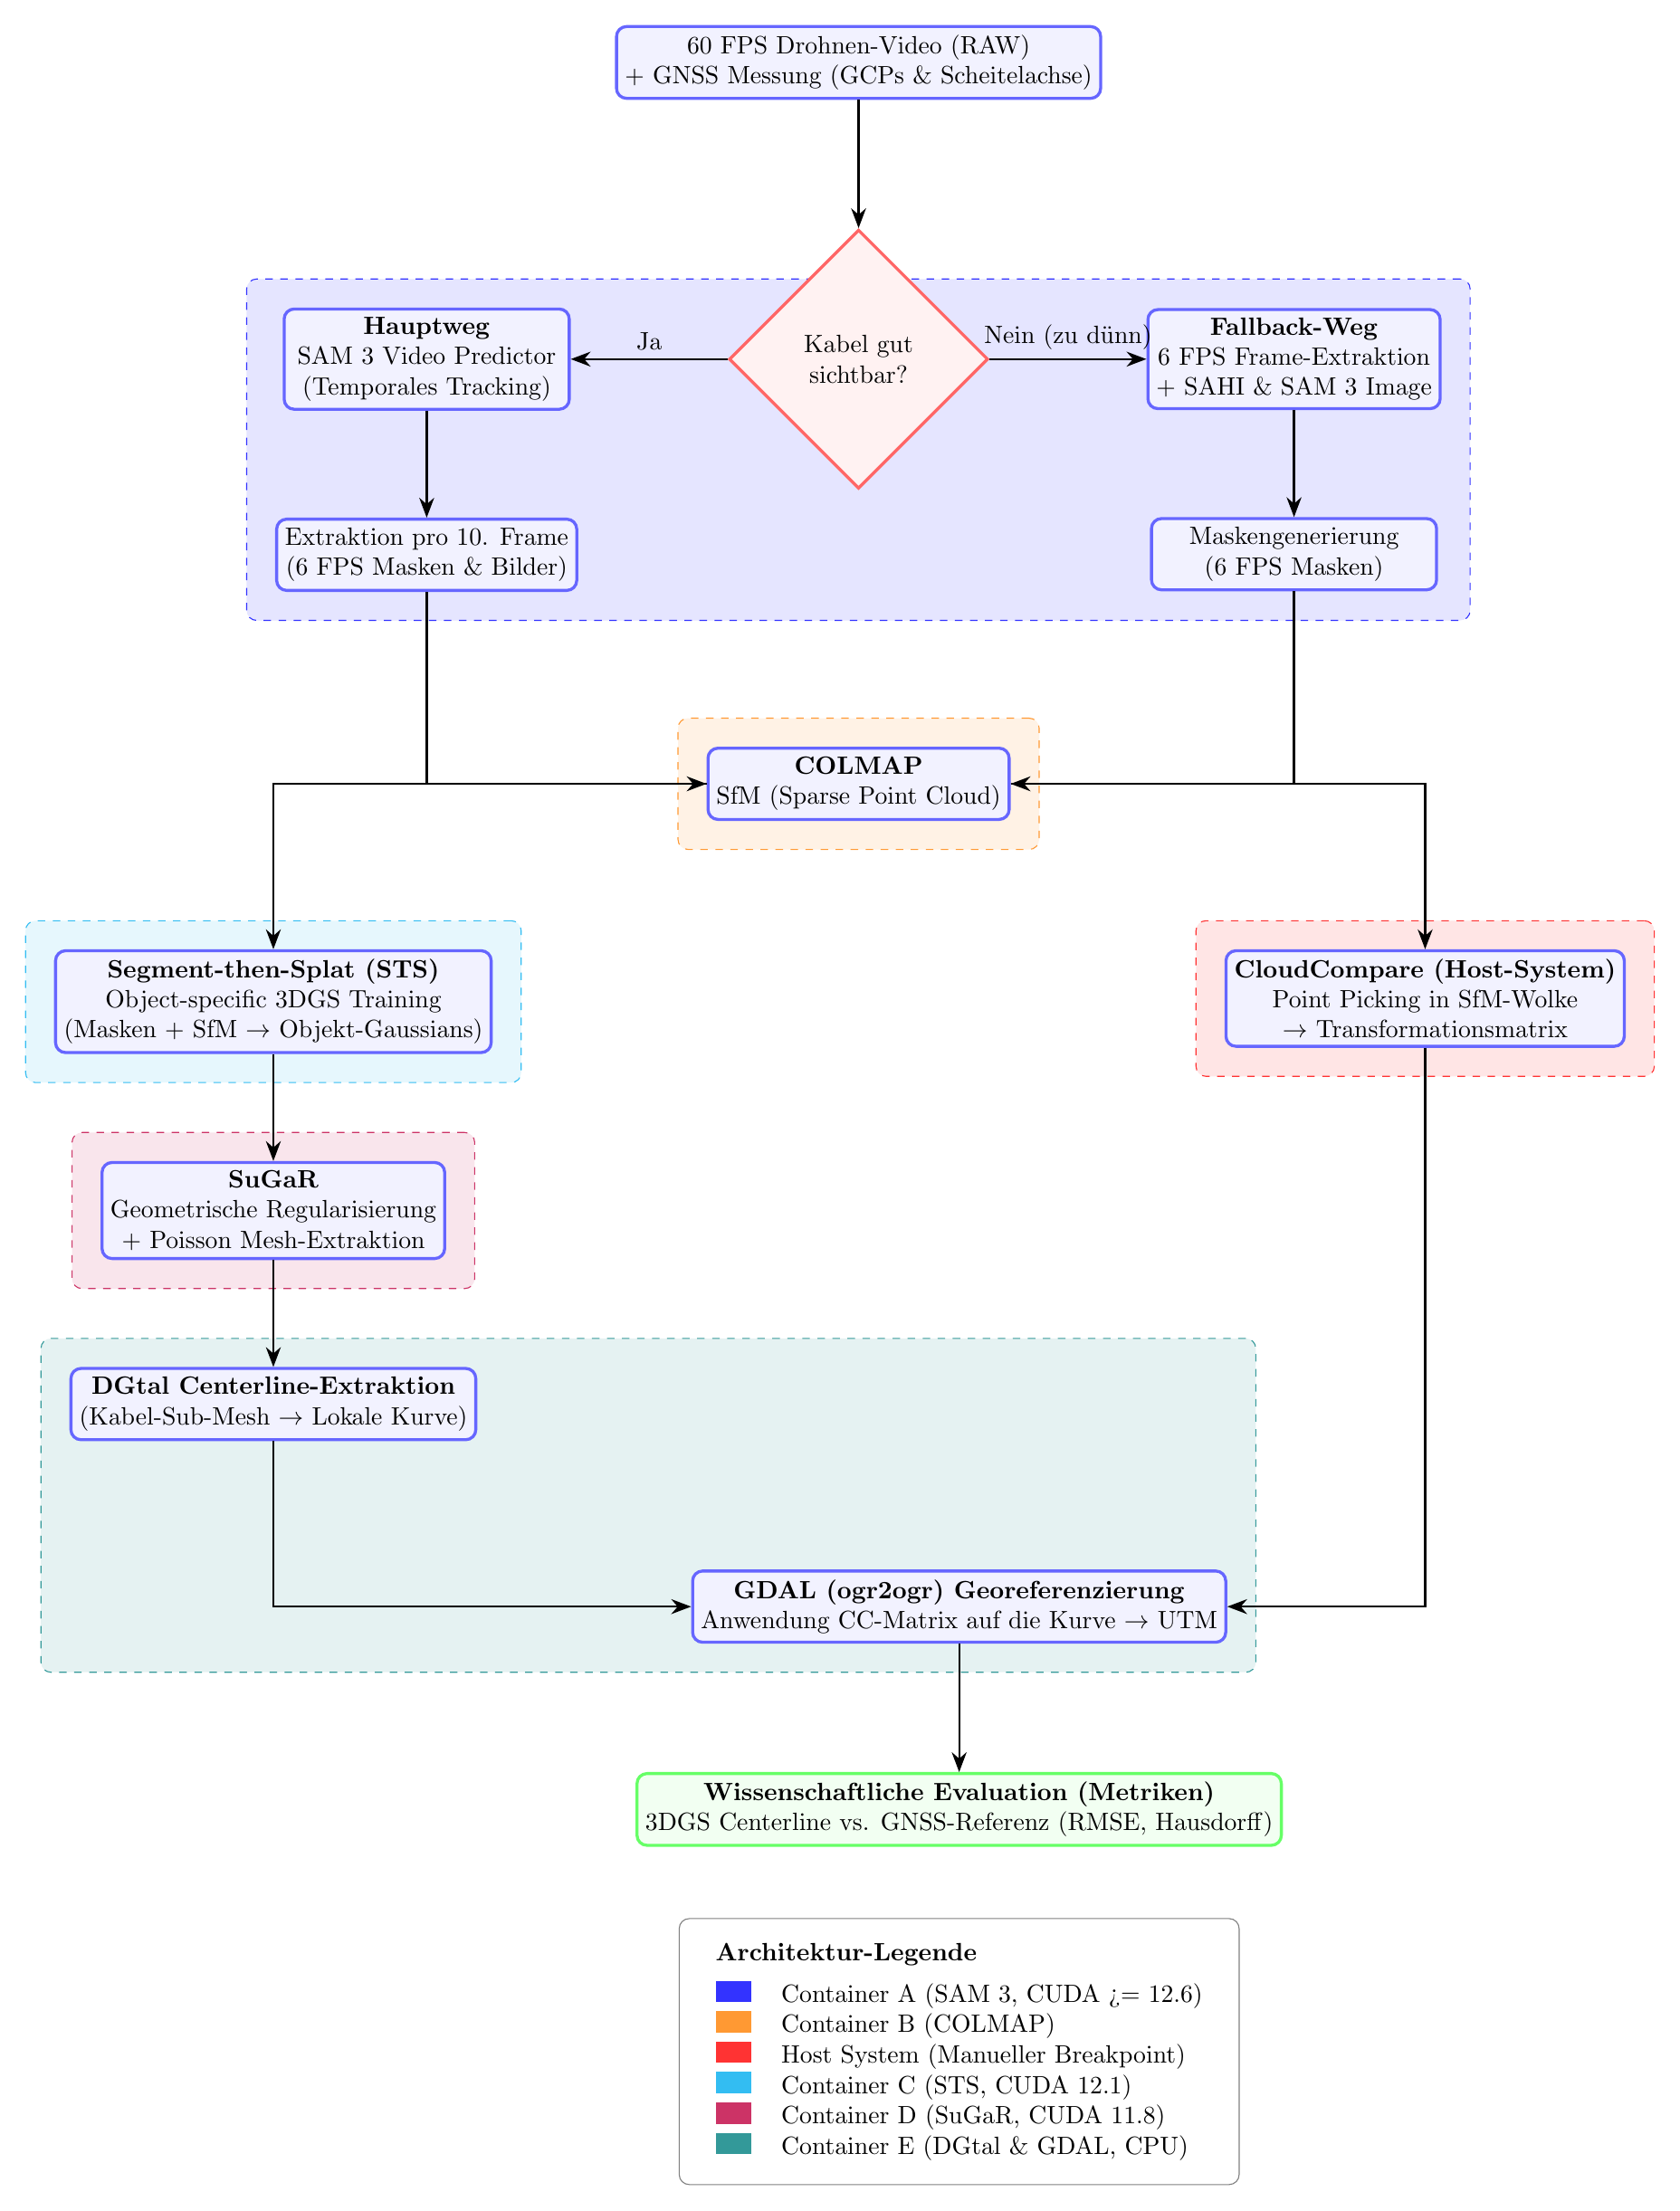
\begin{tikzpicture}[node distance=1.5cm, auto,
                box/.style={rectangle, draw=blue!60, fill=blue!5, very thick, minimum width=4cm, minimum height=1cm, align=center, rounded corners},
                decision/.style={diamond, draw=red!60, fill=red!5, very thick, text width=2.5cm, align=center},
                arrow/.style={-{Stealth[scale=1.2]}, thick},
                container_bg/.style={rectangle, draw, dashed, rounded corners, inner sep=0.4cm}]

            \node[box] (video) {60 FPS Drohnen-Video (RAW)\\+ GNSS Messung (GCPs \& Scheitelachse)};
            \node[decision, below=1.8cm of video] (check) {Kabel gut \\sichtbar?};
            \node[box, left=2.2cm of check] (pathA) {\textbf{Hauptweg}\\SAM 3 Video Predictor\\(Temporales Tracking)};
            \node[box, right=2.2cm of check] (pathB) {\textbf{Fallback-Weg}\\6 FPS Frame-Extraktion\\+ SAHI \& SAM 3 Image};

            \node[box, below=1.5cm of pathA] (extractA) {Extraktion pro 10. Frame\\(6 FPS Masken \& Bilder)};
            \node[box, below=1.5cm of pathB] (extractB) {Maskengenerierung\\(6 FPS Masken)};

            \node[box, below=3.6cm of check] (colmap) {\textbf{COLMAP}\\SfM (Sparse Point Cloud)};

            \node[box, below left=1.8cm and 3.0cm of colmap] (sts) {\textbf{Segment-then-Splat (STS)}\\Object-specific 3DGS Training\\(Masken + SfM $\rightarrow$ Objekt-Gaussians)};
            \node[box, below right=1.8cm and 3.0cm of colmap] (cc) {\textbf{CloudCompare (Host-System)}\\Point Picking in SfM-Wolke\\$\rightarrow$ Transformationsmatrix};

            \node[box, below=1.5cm of sts] (sugar) {\textbf{SuGaR}\\Geometrische Regularisierung\\+ Poisson Mesh-Extraktion};

            \node[box, below=1.5cm of sugar] (dgtal) {\textbf{DGtal Centerline-Extraktion}\\(Kabel-Sub-Mesh $\rightarrow$ Lokale Kurve)};

            \node[box, below right=1.8cm and 3.0cm of dgtal] (final) {\textbf{GDAL (ogr2ogr) Georeferenzierung}\\Anwendung CC-Matrix auf die Kurve $\rightarrow$ UTM};

            \node[box, draw=green!60, fill=green!5, below=1.8cm of final] (eval) {\textbf{Wissenschaftliche Evaluation (Metriken)}\\3DGS Centerline vs. GNSS-Referenz (RMSE, Hausdorff)};

            % Background containers
            \begin{pgfonlayer}{background}
                \node[container_bg, fill=blue!10, draw=blue!80, fit=(pathA) (pathB) (extractA) (extractB)] (contA) {};
                \node[container_bg, fill=orange!10, draw=orange!80, fit=(colmap)] (contB) {};
                \node[container_bg, fill=red!10, draw=red!80, fit=(cc)] (host) {};
                \node[container_bg, fill=cyan!10, draw=cyan!80, fit=(sts)] (contC) {};
                \node[container_bg, fill=purple!10, draw=purple!80, fit=(sugar)] (contD) {};
                \node[container_bg, fill=teal!10, draw=teal!80, fit=(dgtal) (final)] (contE) {};
            \end{pgfonlayer}

            % Legend
            \node[draw=black!50, fill=white, rectangle, rounded corners, anchor=north, inner sep=0.3cm, yshift=-1cm] at (eval.south) {
                \begin{tabular}{ll}
                    \multicolumn{2}{l}{\textbf{Architektur-Legende}}                                \\[1ex]
                    \textcolor{blue!80}{\rule{0.5cm}{0.3cm}}   & Container A (SAM 3, CUDA >= 12.6)  \\
                    \textcolor{orange!80}{\rule{0.5cm}{0.3cm}} & Container B (COLMAP)               \\
                    \textcolor{red!80}{\rule{0.5cm}{0.3cm}}    & Host System (Manueller Breakpoint) \\
                    \textcolor{cyan!80}{\rule{0.5cm}{0.3cm}}   & Container C (STS, CUDA 12.1)       \\
                    \textcolor{purple!80}{\rule{0.5cm}{0.3cm}} & Container D (SuGaR, CUDA 11.8)     \\
                    \textcolor{teal!80}{\rule{0.5cm}{0.3cm}}   & Container E (DGtal \& GDAL, CPU)   \\
                \end{tabular}
            };

            \draw[arrow] (video) -- (check);
            \draw[arrow] (check) -- node[above] {Ja} (pathA);
            \draw[arrow] (check) -- node[above] {Nein (zu dünn)} (pathB);
            \draw[arrow] (pathA) -- (extractA);
            \draw[arrow] (pathB) -- (extractB);
            \draw[arrow] (extractA) |- (colmap);
            \draw[arrow] (extractB) |- (colmap);
            \draw[arrow] (colmap) -| (sts);
            \draw[arrow] (colmap) -| (cc);
            \draw[arrow] (sts) -- (sugar);
            \draw[arrow] (sugar) -- (dgtal);
            \draw[arrow] (dgtal) |- (final);
            \draw[arrow] (cc) |- (final);
            \draw[arrow] (final) -- (eval);

        \end{tikzpicture}
    }
    \caption{Microservice-Architektur (v4): 5-Container-Pipeline mit Segment-then-Splat für objektspezifisches Training und SuGaR für geometrisches Meshing.}
\end{figure}

\section{Anhang: Single Source of Truth (SSOT) -- Pipeline Installation}
Dieses Dokument dient als zentrale Wahrheit (SSOT) für die Installation und Orchestrierung der gesamten 5-Container-Pipeline. Es fasst alle Hard- und Software-Abhängigkeiten zusammen, um Reproduzierbarkeit zu gewährleisten.

\subsection*{Reproduzierbare LaTeX-Kompilation}
Auf dem Ubuntu-Host muss keine lokale LaTeX-Installation vorhanden sein. Der
offizielle MiKTeX-Docker-Workflow ist grundsätzlich geeignet:

\begin{verbatim}
docker run -ti \
  -v miktex:/var/lib/miktex \
  -v "$(pwd)":/miktex/work \
  -e MIKTEX_UID="$(id -u)" \
  miktex/miktex:essential pdflatex Expose_PA_BA.tex
\end{verbatim}

Mit dem am 04.08.2026 verfügbaren MiKTeX-Image $23.10$ schlug dieser Aufruf
jedoch beim Aufbau von \texttt{pdflatex.fmt} fehl, weil das aus dem gewählten
Paket-Repository geladene \texttt{miktex-latex}-Paket die erwartete
\texttt{pdflatex.ini} nicht enthielt. Als reproduzierbarer Fallback wurde
deshalb ein TeX-Live-Container erfolgreich verifiziert:

\begin{verbatim}
docker run --rm -i \
  --user "$(id -u):$(id -g)" \
  -e HOME=/tmp \
  -e TEXMFVAR=/tmp/texlive-var \
  -e TEXMFCONFIG=/tmp/texlive-config \
  -e TEXMFHOME=/tmp/texlive-home \
  -v "$(pwd)":/work -w /work \
  texlive/texlive:latest-small \
  pdflatex -file-line-error -interaction=nonstopmode \
  -halt-on-error Expose_PA_BA.tex
\end{verbatim}

Der TeX-Live-Aufruf erzeugt die PDF sowie die LaTeX-Hilfsdateien im aktuellen
\texttt{docs/}-Verzeichnis, ohne Root-Dateien im Projekt anzulegen. Nach
inhaltlichen Aenderungen sollte der Aufruf mindestens einmal, bei geaenderten
Querverweisen zweimal ausgefuehrt werden. Warnungen wie \textit{Overfull hbox}
sind Layoutwarnungen; ein nicht-null Exit-Code ist dagegen ein echter
Kompilationsfehler.

\subsection*{Hardware-Grundvoraussetzungen}
\begin{itemize}[noitemsep]
    \item \textbf{GPU:} CUDA-kompatible Nvidia GPU (Compute Capability 7.0+).
    \item \textbf{VRAM:} 24 GB (erforderlich, um in Paper-Evaluations-Qualität zu trainieren).
    \item \textbf{OS:} Windows 10/11 mit WSL2 oder natives Ubuntu Linux 22.04.
\end{itemize}

\subsection*{Container A: SAM 3 (Segmentierung)}
Zuständig für die 2D-Maskierung des Drohnenvideos. Dieser Container nutzt modernste Meta-Abhängigkeiten.

\textbf{Requirements (laut offizieller Vorgabe):}
\begin{itemize}[noitemsep]
    \item Python 3.10 or higher
    \item PyTorch 2.4 or higher (im Setup wird PyTorch mit der passenden CUDA-Laufzeitumgebung installiert)
    \item CUDA-kompatible GPU mit CUDA >= 12.6
\end{itemize}

\textbf{Implementierungsentscheidung: Docker vs. Conda}\\
Für die Ausführung der SAM 3.1 Codebasis wurde konzeptionell von einer reinen lokalen Conda-Umgebung Abstand genommen. Stattdessen läuft SAM 3.1 vollständig in einem dedizierten Docker-Container (\texttt{sam3-preprocess}).

\textbf{Gründe gegen Conda und für Docker:}
\begin{enumerate}[noitemsep]
    \item \textbf{CUDA-Konflikte:} SAM 3.1 verlangt moderne PyTorch-Versionen (z.\,B. 2.7.0 mit CUDA 12.6) und greift auf experimentelle C++ Extensions (\texttt{sam3\_cu}) zurück. In einer lokalen Anaconda-Umgebung kommt es hier mit den bestehenden CUDA 11.8 Treibern von COLMAP/SuGaR ständig zu "Layer Mismatches" und Kompilierungsfehlern. Docker kapselt die CUDA 12.6 Abhängigkeiten sauber vom Host-System ab.
    \item \textbf{Abhängigkeits-Knoten (Dependency Hell):} Das SAM 3.1 Release benötigt tiefgreifende Bibliotheken (\texttt{pycocotools}, \texttt{einops}, \texttt{timm}), die nativ im Container über \texttt{apt-get} und \texttt{pip} verlässlich zusammengestellt werden.
    \item \textbf{Hardware-Starvation (Host-Safety):} Das Laden von SAM 3.1 in Full-HD (\texttt{sam3.1\_multiplex.pt}) absorbiert immense RAM- und CPU-Ressourcen beim Instanziieren des Video-Predictors. Im Container können via \texttt{docker-compose.yml} die CPU-Berechnungen strikt gedrosselt werden (\texttt{OMP\_NUM\_THREADS=8}), um Systemabstürze effektiv zu verhindern. Ein VRAM- und RAM-Offloading ist zusätzlich im inferierenden Python-Skript konfiguriert.
    \item \textbf{Hugging Face Token-Sicherheit:} Über Docker-Secrets (\texttt{.env} / \texttt{HF\_TOKEN}) wird die Authentifizierung für Gated Models sicher gehandhabt, ohne lokale Systemumgebungen zu belasten.
\end{enumerate}

\textbf{Installationsablauf (Docker):}\\
Die Bereitstellung erfolgt vollautomatisch über das dedizierte \texttt{Dockerfile} auf Basis von \texttt{pytorch/pytorch:2.7.0-cuda12.6-cudnn9-devel}. Dies klont das offizielle Repository, baut die C++ Extensions und cacht über das Hugging Face Hub das 3.5\,GB schwere Multiplex-Gewicht persistent ins Host-Volume.

\textbf{Ausführung \& Masken-Export (Python API):}\\
Hier ist das Python-Skript zur temporalen Propagation des Kabel-Prompts im Video. Da der SAM 3 Video Predictor im Tracking-Modus aus Konsistenzgründen nur eine einzelne, eindeutige Maske pro Frame propagiert (und nicht die drei hierarchischen Skalen des Image Predictors), generiert das Skript die für das Curriculum-Learning von Segment-then-Splat (STS) benötigten Stufen (\texttt{small}, \texttt{middle}, \texttt{default}) künstlich über morphologische Bildoperationen (Erosion und Dilation):
\begin{verbatim}
import os
import cv2
import numpy as np
from PIL import Image
from sam3.model_builder import build_sam3_video_predictor

# 1. Video Predictor auf GPU 0 initialisieren
predictor = build_sam3_video_predictor(gpus_to_use=[0])

# 2. Session mit dem Drohnen-Video starten
video_path = "/data/video.mp4"
response = predictor.handle_request(
    request=dict(type="start_session", resource_path=video_path)
)
session_id = response["session_id"]

# 3. Prompt setzen (z. B. Punkt-Prompt auf das Kabel in Frame 0)
predictor.handle_request(
    request=dict(
        type="add_prompt",
        session_id=session_id,
        frame_index=0,
        points=[[1024, 768]],  # Beispielkoordinaten auf dem Kabel
        labels=[1]
    )
)

# 4. Stream-Propagation & Multi-Scale Export via Morphologie
output_dir = "/data/masks"
os.makedirs(output_dir, exist_ok=True)

# Definiere Kernel für Erosion und Dilation (Größe auf Kabeldurchmesser anpassen)
kernel = np.ones((5, 5), np.uint8)

# propagate_in_video liefert einen Generator
for response in predictor.handle_stream_request(
    request=dict(type="propagate_in_video", session_id=session_id)
):
    frame_idx = response["frame_index"]
    outputs = response["outputs"]
    obj_ids = outputs["out_obj_ids"]
    binary_masks = outputs["out_binary_masks"]  # Shape: [num_objects, H, W]

    # Erzeuge einen Unterordner pro Frame-Index
    frame_dir = os.path.join(output_dir, f"frame_{frame_idx:05d}")
    os.makedirs(frame_dir, exist_ok=True)

    for idx, obj_id in enumerate(obj_ids):
        mask = binary_masks[idx]  # Boolesches Array [H, W]
        if mask.any():
            # Konvertierung: True -> 255, False -> 0
            mask_uint8 = (mask * 255).astype(np.uint8)
            
            # 1. Middle (Original)
            img_middle = Image.fromarray(mask_uint8)
            img_middle.save(os.path.join(frame_dir, "middle.png"))
            
            # 2. Small (Erodiert für den stabilen Kabelkern)
            mask_small = cv2.erode(mask_uint8, kernel, iterations=1)
            img_small = Image.fromarray(mask_small)
            img_small.save(os.path.join(frame_dir, "small.png"))
            
            # 3. Default (Dilatiert für den Sicherheitsrand)
            mask_default = cv2.dilate(mask_uint8, kernel, iterations=1)
            img_default = Image.fromarray(mask_default)
            img_default.save(os.path.join(frame_dir, "default.png"))

# 5. Session sauber schließen
predictor.handle_request(
    request=dict(type="close_session", session_id=session_id)
)
\end{verbatim}

\subsection*{Container B: COLMAP (Structure from Motion)}
Generiert die Kameraposen und die Sparse Point Cloud aus den unmaskierten
Originalbildern. Die unmaskierten Hintergrund- und Anker-Features sind fuer
die stabile Orientierung duenn strukturierter Objekte und fuer das spaetere
GCP-Picking erforderlich. Die Docker-Pipeline verwendet in der Projektarbeit
weiterhin bewusst das offizielle Image \texttt{colmap/colmap:latest}; die
frueher dokumentierte Bezeichnung \texttt{4.0.4-cuda} ist aktuell nicht als
Docker-Hub-Tag verfuegbar und bleibt eine spaetere Versionsoption.

\textbf{Quellen \& Docker-Image:}
\begin{itemize}[noitemsep]
    \item \textbf{Releases:} \url{https://github.com/colmap/colmap/releases}
    \item \textbf{Docker-Image:} \texttt{docker pull colmap/colmap:latest}
\end{itemize}

\textbf{Ausführung \& PLY-Export (für CloudCompare):}\\
Da COLMAP die Punktwolke standardmäßig in einem proprietären Binärformat (\texttt{.bin}) speichert, welches von CloudCompare nicht direkt gelesen werden kann, wird die Punktwolke direkt im Anschluss an die Rekonstruktion über den \texttt{model\_converter} in eine standardisierte \texttt{.ply}-Datei exportiert. Um eine geometrische Verformung der Punktwolke (ebene Entartung/Kollaps) während der Rekonstruktion unkalibrierter Drohnenbilder zu verhindern, wird die Parametrisierung basierend auf modernsten Photogrammetrie-Workflows angepasst (\texttt{SIMPLE\_RADIAL} Kameramodell, erzwungenes gemeinsames Objektiv via \texttt{single\_camera 1} und sequentielles Matching).

\begin{verbatim}
# 1. Feature-Extraktion (Kameramodell einschränken & gleiches Objektiv forcieren)
colmap feature_extractor \
    --database_path /data/scene/database.db \
    --image_path /data/scene/images \
    --ImageReader.camera_model SIMPLE_RADIAL \
    --ImageReader.single_camera 1

# 2. Keypoint-Matching (Sequentiell mit Overlap statt Exhaustive für Videoüberhang)
colmap sequential_matcher \
    --database_path /data/scene/database.db \
    --SequentialMatching.overlap 15

# 3. Structure-from-Motion (Sparse Reconstruction)
mkdir -p /data/scene/sparse
colmap mapper \
    --database_path /data/scene/database.db \
    --image_path /data/scene/images \
    --output_path /data/scene/sparse

# 4. Export der Punktwolke als PLY-Format
colmap model_converter \
    --input_path /data/scene/sparse/0 \
    --output_path /data/scene/sparse/points3D.ply \
    --output_type PLY
\end{verbatim}

\textbf{Hintergrund zur mathematischen Optimierung (für „Dummis“ erklärt):}\\
Wenn wir ein Drohnenvideo Frame-für-Frame in COLMAP einspeisen, stehen wir vor zwei massiven mathematischen Hürden:
\begin{enumerate}[noitemsep]
    \item \textbf{Die Overfitting-Falle (Zu viele Freiheitsgrade):} Wenn wir COLMAP ein extrem komplexes Kameramodell (wie \texttt{OPENCV}) geben, versucht der Algorithmus, für jedes der hunderte Bilder Brennweiten und Objektivkrümmungen völlig unabhängig voneinander zu schätzen. Das führt zu einer geometrischen Katastrophe: COLMAP „schummelt“ mathematisch, verbiegt die Parameter extrem und presst die gesamte 3D-Welt flach wie eine Flunder auf eine einzige Ebene zusammen, um Restfehler zu minimieren. Mit \texttt{SIMPLE\_RADIAL} verbieten wir diese Schummelei, indem wir nur noch vier physikalische Kern-Parameter zulassen. Gleichzeitig zentrieren wir über \texttt{--ImageReader.single\_camera 1} alle Rechnungen auf genau \textit{ein} einziges, geteiltes Objektiv.
    \item \textbf{Die Basislinien-Falle (Fast-parallele Sehstrahlen):} Wenn zwei aufeinanderfolgende Bilder nur Millisekunden auseinander liegen, bewegt sich die Drohne kaum fort. Die Sehstrahlen der Kameras schneiden sich unter einem extrem spitzen Winkel ($0^\circ$). COLMAP kann die Tiefe dadurch nicht verlässlich berechnen und flacht die Punktwolke ab. Indem wir über \texttt{SAM3\_FRAME\_STEP} künstlich nur jedes z.\,B. 5. oder 10. Bild rekonstruieren, vergrößern wir den physischen Abstand (die Basislinie) zwischen den Kamera-Standorten. Dadurch schneiden sich die Sehstrahlen in einem gesunden, steilen Dreieck und zaubern eine plastische, tiefe, dreidimensionale 3D-Struktur hervor.
    \item \textbf{Die Treffsicherheits-Falle (Falsche Übereinstimmungen):} Das standardmäßige \texttt{exhaustive\_matcher} vergleicht jedes Bild mit absolut jedem anderen Bild. Bei sich wiederholenden Texturen (z.\,B. Gleisen, Rohren oder Asphaltmustern) führt das zu fatalen Fehlverknüpfungen (False Loop Closures). Indem wir auf den \texttt{sequential\_matcher} mit einem Overlap von 15 Frames umschalten, vergleicht COLMAP Bilder nur noch mit ihren unmittelbaren zeitlichen Nachbarn (im Video naheliegend). Das ist nicht nur hunderte Male schneller, sondern schützt die 3D-Punktwolke hochgradig effektiv vor geometrischer Verwerfung.
    \item \textbf{Die CLI-Versions-Falle (Veraltete Befehle):} Beim Upgrade auf modernere, offizielle Docker-Images (wie \texttt{colmap/colmap:latest} ab Version \texttt{4.0}) scheitern klassische, ältere Skripte an deprecated Parametern. Parameter wie \texttt{--SiftExtraction.use\_gpu} oder \texttt{--SiftExtraction.max\_image\_size} wurden aus dem CLI-Befehlssatz gestrichen, da die moderne CUDA-Hardware-Beschleunigung und das Auto-Resizing heute vollautomatisch und optimal aufeinander abgestimmt nativ im Kernel von COLMAP implementiert sind. Das Entfernen dieser Parameter garantiert die reibungslose Ausführung auf modernen GPGPU-Knoten.
    \item \textbf{Die CHOLMOD-Numerik-Falle und Levenberg-Marquardt-Instabilität:} \\
          Während der Bildregistrierung im \texttt{colmap mapper} taucht wiederholt die Warnmeldung auf: \\
          \texttt{Linear solver failure. Failed to compute a step: CHOLMOD warning: Matrix not positive definite.} \\
          **Wissenschaftliche Erklärung:** COLMAP nutzt für die Bündelblockausgleichung (\textit{Bundle Adjustment} / gemeinsame Optimierung von 3D-Punkten und Kameraposen) standardmäßig den quadratischen Optimierungsalgorithmus nach **Levenberg-Marquardt (LM)** via \textit{Ceres-Solver}. Um die Schrittweite $\Delta x$ zu berechnen, löst Ceres in jeder Iteration das linearisierte Normalgleichungssystem:
          \[
          (J^{\top} J + \mu I) \Delta x = -J^{\top} f
          \]
          wobei $J$ die Jacobi-Matrix der partiellen Ableitungen, $\mu$ der Dämpfungsparameter und $f$ der Vektor der Reprojektionsfehler ist. Die Koeffizientenmatrix $H = J^{\top} J + \mu I$ ist theoretisch symmetrisch und positiv-definit (alle Eigenwerte $> 0$), was die Nutzung der sehr schnellen und numerisch stabilen **Cholesky-Zerlegung** (implementiert über die SuiteSparse-Bibliothek \textit{CHOLMOD}) erlaubt. \\
          In unserem Testszenario (weißes, kontrastarmes Tischtuch mit wenigen, verrauschten Punktkorrespondenzen) degeneriert das System jedoch geometrisch. Wenn künstlich verrauschte oder geometrisch kollineare Strahlen geschnitten werden sollen, verliert die Jacobi-Matrix ihren vollen Spaltenrang. Dadurch kollabiert die Matrix $J^{\top} J$ stellenweise zu einer singulären Matrix (Rangdefekt / unvollständiges Gleichungssystem mit unendlich vielen Scheinlösungen). Die Dämpfung $\mu$ ist temporär zu klein, um dies auszugleichen, wodurch die Matrix $H$ numerisch nicht-positiv-definit wird (einige Eigenwerte schrumpfen auf $\le 0$). \\
          **Numerische Konsequenz:** CHOLMOD bricht die Cholesky-Zerlegung $H = L L^{\top}$ an einer Division durch Null (oder Wurzel aus einer negativen Zahl) ab. Ceres fängt diese Warnung jedoch intern robust ab: Das System vergrößert im nächsten Schritt den Dämpfungskoeffizienten $\mu$ drastisch (Gefälle wechselt vom Newton-Schritt in Richtung des steilsten Abstiegs / Gradient Descent). Dadurch wird die Matrix wieder numerisch stabilisiert und der Schritt wiederholt. Die Warnung ist somit **ein klarer Indikator für extreme Texturarmut** der Szene, führt jedoch dank der internen Dämpfungsdynamik von Ceres *nicht* zum Absturz der gesamten Rekonstruktion, solange genügend gesunde Bildbereiche verbleiben.
\end{enumerate}

\textit{Breakpoint:} Nach diesem Schritt pausiert das Master-Skript automatisch. Die erzeugte Datei \texttt{points3D.ply} wird auf dem Host-System in CloudCompare geladen, um die manuelle Georeferenzierung via GCP-Point-Picking durchzuführen. Nach dem Speichern der Transformationsmatrix wird das Skript fortgesetzt.

\subsection*{Container C: Segment-then-Splat (Object-specific 3DGS)}
Führt das objektspezifische 3DGS-Training durch. STS weist jedem initialen COLMAP-Gaussian eine Object-ID zu (basierend auf den SAM 3 Masken) und trainiert mit dem nativen Object-specific Loss ($\mathcal{L}_{obj}$). Das intern vorgesehene AutoSeg-SAM2 wird vollständig deaktiviert und durch die externen SAM 3 Masken aus Container A ersetzt. Hierfür wird der Dataloader (z. B. in \texttt{scene/dataset\_readers.py} oder \texttt{scene/cameras.py}) so angepasst, dass er pro Frame die drei Masken-Dateien (\texttt{small.png}, \texttt{middle.png}, \texttt{default.png}) einliest und in das Dictionary \texttt{viewpoint\_cam.object\_masks} einspeist.

\textbf{Requirements (Docker-Umgebung):}
\begin{itemize}[noitemsep]
    \item \textbf{Base Image:} \texttt{nvidia/cuda:12.1.0-devel-ubuntu22.04}
    \item Python 3.10, PyTorch 2.3.1 mit CUDA 12.1
    \item 24 GB VRAM
\end{itemize}

\textbf{Installationsablauf:}
\begin{verbatim}
git clone https://github.com/luyr/Segment-then-Splat --recursive
cd Segment-then-Splat

conda create -n segment_then_splat python=3.10
conda activate segment_then_splat
pip install torch==2.3.1 torchvision==0.18.1 torchaudio==2.3.1 \
    --index-url https://download.pytorch.org/whl/cu121
pip install -r requirements.txt --no-build-isolation
\end{verbatim}

\textbf{Anpassung des Dataloaders und Trainingsablauf:}
Im Datensatz-Reader wird die folgende Logik implementiert, um die Maskentensoren direkt zu laden:
\begin{verbatim}
# Pseudo-Code zur Anpassung des Kamera-Ladevorgangs:
import torch
from PIL import Image

def load_object_masks(frame_dir):
    scales = ["small", "middle", "default"]
    object_masks = {}
    for scale in scales:
        mask_path = os.path.join(frame_dir, f"{scale}.png")
        if os.path.exists(mask_path):
            # Graustufen laden, Normalisieren und als Boolean-Tensor konvertieren
            mask_img = Image.open(mask_path).convert("L")
            mask_np = np.array(mask_img) > 127
            mask_tensor = torch.from_numpy(mask_np).bool() # Shape: [H, W]
            object_masks[scale] = [mask_tensor]
        else:
            object_masks[scale] = []
    return object_masks

# Zuweisung zur viewpoint_cam während der Szenen-Initialisierung:
# viewpoint_cam.object_masks = load_object_masks(f"/data/masks/frame_{frame_idx:05d}")
\end{verbatim}

\textbf{Ausführung des Trainings:}
\begin{verbatim}
# 1. Object-specific Initialization (Zuweisung der initialen SfM-Punkte)
# STS prüft anhand der default/middle/small Masken die Punkt-Sichtbarkeiten
python ./helpers/object_specific_initialization.py \
    --scene_root /data/scene/

# 2. Training mit dem geänderten Dataloader und Object-specific Loss
python train.py -s /data/scene/ -m /data/output \
    --eval --iterations 40000 \
    --num_sample_objects 3 \
    --densify_until_iter 20000 \
    --partial_mask_iou 0.3
\end{verbatim}

\textbf{Wichtiger Hinweis:} Durch die Entkopplung der Maskenberechnung läuft die CUDA-spezifische Optimization in Container C völlig autark von den CUDA-Anforderungen des SAM 3 Frontends in Container A.

\subsection*{Container D: SuGaR (Geometrische Regularisierung \& Meshing)}
Lädt den vortrainierten STS-Checkpoint und wendet die geometrische Regularisierung (DN-Consistency, Normal Alignment) sowie Poisson Surface Reconstruction an. Dies ist der sensitivste Container bezüglich CUDA-Versionen.

\textbf{Exkurs: Conda innerhalb von Docker}\\
Obwohl Docker bereits das Betriebssystem isoliert und Conda somit theoretisch redundant wäre, wird Miniconda in diesem Container explizit genutzt. Der Grund: 3DGS-Repositories (wie SuGaR) setzen stark auf vorkompilierte Conda-Binaries (z.B. \texttt{pytorch-cuda}) und exakte Paket-Versionen. Durch die strikte Nutzung von Conda im Docker-Container werden fatale C++ Kompilierungsfehler beim Rasterizer-Modul präventiv vermieden.

\textbf{Requirements (Docker-Umgebung):}
\begin{itemize}[noitemsep]
    \item \textbf{Base Image:} \texttt{nvidia/cuda:11.8.0-devel-ubuntu22.04} (Dieses Image bringt das kompatible CUDA 11.8 SDK direkt mit).
    \item \textbf{C++ Compiler:} Installation via \texttt{apt-get install build-essential} (installiert GCC/G++, was unter Linux Visual Studio ersetzt und garantiert mit CUDA 11.8 kompatibel ist).
    \item 24 GB VRAM (erforderlich, um in Paper-Evaluations-Qualität zu trainieren).
\end{itemize}

\textbf{Installationsablauf (Dockerfile-Struktur):}
\begin{verbatim}
# 1. Base Image mit CUDA 11.8 & GCC
FROM nvidia/cuda:11.8.0-devel-ubuntu22.04

# 2. System-Abhängigkeiten installieren
ENV DEBIAN_FRONTEND=noninteractive
RUN apt-get update && apt-get install -y \
    build-essential \
    git \
    wget \
    curl \
    libgl1-mesa-glx \
    libglib2.0-0 \
    && rm -rf /var/lib/apt/lists/*

# 3. Miniconda installieren
RUN wget https://repo.anaconda.com/miniconda/Miniconda3-latest-Linux-x86_64.sh -O miniconda.sh && \
    bash miniconda.sh -b -p /opt/conda && \
    rm miniconda.sh
ENV PATH=/opt/conda/bin:$PATH

# 4. Conda Environment anlegen und Shell konfigurieren
RUN conda create --name sugar -y python=3.9
SHELL ["conda", "run", "-n", "sugar", "/bin/bash", "-c"]

# 5. PyTorch & CUDA 11.8 Bibliotheken installieren
RUN conda install pytorch==2.0.1 torchvision==0.15.2 torchaudio==2.0.2 \
    pytorch-cuda=11.8 -c pytorch -c nvidia -y && \
    conda install -c fvcore -c iopath -c conda-forge fvcore iopath -y && \
    conda install pytorch3d==0.7.4 -c pytorch3d -y && \
    conda install -c plotly plotly -y && \
    conda install -c conda-forge rich plyfile==0.8.1 jupyterlab nodejs ipywidgets -y

# 6. Repositories klonen und Submodule kompilieren
WORKDIR /workspace
RUN git clone https://github.com/Anttwo/SuGaR.git && \
    cd SuGaR && \
    pip install open3d PyMCubes && \
    pip install -e . && \
    cd gaussian_splatting/submodules/diff-gaussian-rasterization/ && \
    pip install -e . && \
    cd ../simple-knn/ && \
    pip install -e .

# Conda-Umgebung im PATH systemweit als Standard setzen
ENV PATH=/opt/conda/envs/sugar/bin:$PATH
\end{verbatim}

\textbf{Details zur Build-Dauer und Kompilierungskomplexität (Container D):}\\
In der praktischen Umsetzung stellte der Docker-Build für SuGaR eine signifikante Hürde dar, die mehrere Optimierungszyklen erforderte:
\begin{enumerate}[noitemsep]
    \item \textbf{Explizite CUDA-Architektur-Spezifikation (\texttt{TORCH\_CUDA\_ARCH\_LIST}):} Um die Ausführbarkeit auf einer breiten Hardwarelandschaft (z.\,B. RTX 30er, 40er, Server-GPUs) abzusichern, mussten mehrere CUDA-Architekturen (\texttt{"7.0;7.5;8.0;8.6;8.9;9.0"}) explizit beim Build hinterlegt werden. Der NVCC-Compiler kompiliert die C++ Extensions von \texttt{diff-gaussian-rasterization} und \texttt{simple-knn} für jede Architektur einzeln, was die Kompilierungszeit erheblich verlängert.
    \item \textbf{Conda-Umgebung und Build-Isolation (\texttt{-{}-no-build-isolation}):} Standardmäßig isoliert \texttt{pip} Builds in temporären virtuellen Umgebungen. Weil darin jedoch kein Zugriff auf die installierten PyTorch- und CUDA-Laufzeitbibliotheken von Conda besteht, kommt es zu fatalen Kompilierungsabbrüchen (z.\,B. bzgl. fehlender \texttt{torch}-Vektoren). Erst durch Hinzufügen von \texttt{-{}-no-build-isolation} greift der Build-Prozess direkt auf den vorkonfigurierten Conda-Compiler-Stack zu.
    \item \textbf{Parallelisierung via \texttt{ninja-build}:} Ohne eine parallele Kompilierungssteuerung fallen manche Python-Installer auf serielle Single-Thread-Kompilierung zurück, was zu extremen Timeouts oder Speicherüberläufen führt. Das Vorinstallieren des systemweiten Compilers \texttt{ninja-build} im Docker-Base-Image ermöglichte hierbei die maximal parallele Lastverteilung auf alle CPU-Kerne.
\end{enumerate}

\subsubsection*{Maskenkonsistente SuGaR-Optimierung und objektbezogene Mesh-Extraktion}
\textbf{Ausgangsproblem und theoretische Konsequenz:} Die Originalimplementierung von SuGaR verwendet für den photometrischen Rekonstruktionsverlust die vollständigen RGB-Trainingsbilder. Eine alleinige Filterung der 3DGS-Punktwolke auf Kabel-Gaussians reicht daher nicht aus: Der Optimierer würde ein objektisoliertes Modell gegen Pixel des gesamten Bildes -- einschließlich Boden, Graben und Hintergrund -- anpassen. Das erzeugt einen Zielkonflikt zwischen 3D-Initialisierung und Bildsupervision und kann trotz optisch überzeugender 3DGS-Renderings zu geometrisch falschen oder aufgeblähten Meshes führen. Deshalb werden Full-Scene-Baseline und Objektpfad strikt getrennt. Die Standarddatei \texttt{point\_cloud.ply} bleibt eine vollständige Referenz; \texttt{point\_cloud\_filtered.ply} bewahrt die echte Filterung mit Originalopazitäten, während \texttt{point\_cloud\_filtered\_opacity999999.ply} als bewusst geometrieorientierter Eingang in einen privaten maskenkonsistenten Objekt-Checkpoint kopiert wird.

\textbf{Maskenhierarchie und Verluste:} Für jede registrierte Kamera wird die SAM-3-Maske über den Bildnamen aufgelöst. Die aktuelle Datenprüfung bestätigte für alle 699 Kameras nichtleere Masken der Stufen \texttt{default}, \texttt{middle} und \texttt{small} bei einer Bildgröße von $768 \times 432$ Pixeln. Der RGB-Verlust wird nur auf Vordergrundpixeln $M(p) \in \{0,1\}$ ausgewertet:
\[
\mathcal{L}_{\mathrm{RGB}}^{M} =
\frac{\sum_{p} M(p)\,\ell_{\mathrm{RGB}}(p)}
    {\sum_{p} M(p) + \varepsilon}.
\]
Hierbei kombiniert $\ell_{\mathrm{RGB}}$ den L1-Term mit DSSIM. Für die Depth-Normal Consistency wird die konservativere \texttt{middle}-Maske verwendet, um unsichere Silhouettenränder nicht als Normalenrestriktion zu interpretieren:
\[
\mathcal{L}_{\mathrm{DN}}^{M} =
\frac{\sum_{p} M_{\mathrm{middle}}(p)
\left[1-\mathbf{n}_{\mathrm{depth}}(p)^{\top}\mathbf{n}_{\mathrm{Gauss}}(p)\right]}
    {\sum_{p} M_{\mathrm{middle}}(p) + \varepsilon}.
\]
Beim anschließenden UV-Baking werden nur die von der jeweiligen Kamera als Objekt markierten Rasterpixel in die Texturakkumulation übernommen. Die \texttt{default}-Maske kann dabei um wenige Pixel dilatiert werden, damit geringe Silhouetten- oder Kalibrierungsungenauigkeiten keine sichtbaren Texturlücken erzeugen.

\textbf{Gleiche Ausgangsmasken, unterschiedliche Wirkorte:} Die SAM-Masken werden in der Pipeline mehrfach, jedoch mit unterschiedlicher Funktion verwendet. STS nutzt sie zunächst zur Objektzuordnung der Gaussians und erzeugt daraus \texttt{point\_cloud\_filtered.ply}; die Hochopazitätskopie \texttt{point\_cloud\_filtered\_opacity999999.ply} dient anschließend als Standardinput für die Geometrieoptimierung. Dass diese Wolke in kamera-ausgerichteten Ansichten nahe an der Brille liegt, ist daher ein wichtiges Gegenindiz gegen grobe, frei schwebende Eingabe-Splats. SuGaR verwendet dieselben Ausgangsmasken anschließend erneut als Bildsupervision. Der aktuelle geführte Standard verwendet keine RGB- oder UV-Dilatation; solche Dilatationen bleiben getrennte Ablationen, weil unsichere Silhouetten- oder Hintergrundpixel die Geometrie indirekt beeinflussen können. Der DN-Term verwendet die einmal erodierte \texttt{middle}-Maske ohne zusätzliche Dilatation. Die UV-Maske begrenzt ausschließlich die spätere Farbsammlung im Texturatlas; sie ist kein geometrischer Loss und kann weder Coarse-Mesh noch verfeinerte PLY verändern.

\textbf{Bedeutung der DN-Maske:} DN steht für \emph{Depth-Normal Consistency}. Die DN-Maske enthält keine gemessenen Tiefen oder Normalen und erzeugt auch keine Geometrie. Sie ist eine semantische Pixelgewichtung: \texttt{middle} ist die ursprüngliche SAM-Objektmaske nach einer $5 \times 5$-Erosion und blendet damit den unsicheren Silhouettenrand aus. Für eine Trainingskamera rendert SuGaR eine Tiefenkarte und eine Normalenkarte aus seinen Gaussians. Aus lokalen Tiefendifferenzen wird eine zweite Normale abgeleitet; der DN-Loss bestraft ihre Abweichung von der gerenderten Gaussian-Normale nur innerhalb der \texttt{middle}-Maske und ohne zusätzliche Dilatation. Er nutzt also keine externe Normalenreferenz, sondern erzwingt Selbstkonsistenz der aktuellen Darstellung. Der Bildrand von einem Pixel wird technisch ebenfalls ausgeschlossen, weil dort keine Tiefennormale definiert ist. Im aktuellen Trainer wird dieser Term erst nach Zählerstand $9000$ mit Gewicht $0.05$ aktiviert. Die DN-Maske filtert weder die STS-Eingabewolke noch den UV-Atlas; im Refinement wird sie derzeit gar nicht verwendet.

\textbf{Reproduzierbare Implementierung:} Die Erweiterung liegt als versionsfixierter lokaler SuGaR-Fork unter \texttt{third\_party/SuGaR} vor; der vollständige Ausgangscommit ist zugleich im Dockerfile festgelegt. Während der Entwicklung überlagert die optionale Compose-Datei \texttt{docker-compose.sugar-dev.yml} diesen Quellstand in den bestehenden Containerpfad \texttt{/opt/sugar}; ein wiederholtes Herunterladen oder Neubauen des Images ist damit nicht erforderlich. Der Runner \texttt{run\_masked\_sugar.sh} erzeugt getrennte Ausgabeverzeichnisse, nutzt \texttt{dn\_consistency} und führt die vollständige Kette aus Coarse-Optimierung, Mesh-Extraktion, Refinement und Textur-Export aus. Die geänderten Module wurden kompiliert; der maskierte RGB-Gradient sowie der maskierte Depth-Normal-Pfad wurden mit realen Kamera- und Maskendaten getestet. Ein vollständiger, zeitintensiver Objektlauf mit $699$ Kameras hat inzwischen ein texturiertes OBJ erzeugt; seine geometrische Qualität ist jedoch noch Gegenstand der folgenden Stufenanalyse.

\textbf{Entstehung des Coarse-Meshes:} Der private Objekt-Checkpoint initialisiert SuGaR mit der aus der echten Filterung erzeugten Hochopazitätskopie der STS-Wolke. Die Originalopazitäten bleiben in \texttt{point\_cloud\_filtered.ply} für Diagnostik und Vergleich erhalten; die einheitliche hohe Eingangsopazität ist ausschließlich eine Entscheidung für die geometrische Stützung der Standardroute. Im Coarse-Training werden gerenderte RGB-Bilder gegen die Originalbilder innerhalb der RGB-Maske optimiert. Die aktuelle lokale \texttt{dn\_consistency}-Konfiguration übernimmt den Iterationszähler des geladenen STS-Modells und startet deshalb bei $6999$. Die Angabe $15000$ ist ein Zielwert dieses Zählers, nicht $15000$ zusätzliche Optimierungsschritte; sie entspricht näherungsweise $15000-6999=8001$ Coarse-Updates. Zwischen Zählerstand $7000$ und $9000$ stabilisieren maskierter RGB-Loss und Entropieregularisierung die Darstellung. Nach $9000$ werden zusätzlich die geometrischen SDF-Terme und die Depth-Normal Consistency aktiviert. Letztere vergleicht innerhalb der nicht dilatierten \texttt{middle}-Maske die aus der gerenderten Tiefe abgeleitete Flächennormale mit der Normalenrichtung der Gaussians:
\[
\mathcal{L}_{\mathrm{DN}}^{M} =
\frac{\sum_{p} M_{\mathrm{middle}}(p)
\left[1-\mathbf{n}_{\mathrm{depth}}(p)^{\top}\mathbf{n}_{\mathrm{Gauss}}(p)\right]}
{\sum_{p} M_{\mathrm{middle}}(p)+\varepsilon}.
\]
Der verzögerte Start ist ein lokales Curriculum: Zunächst soll sich die photometrisch passende Dichteverteilung stabilisieren, bevor eine geometrische Normalenrestriktion auf möglicherweise noch unsichere Oberflächen wirkt. Ein Zielwert von $7500$ ergäbe dadurch nur rund $501$ neue Updates und noch keinen DN-Term; $12000$ ergibt rund $5001$ neue Updates, davon etwa $3000$ nach Aktivierung der DN- und SDF-Terme. Für den segmentierten Projektarbeitsstandard wird deshalb bewusst der Zielwert $9000$ verwendet: Die DN-/SDF-Phase beginnt erst bei $iteration>9000$ und wird damit nicht benötigt. Die frühere Eingabeuntergrenze $9001$ wurde aufgehoben; Werte über $9000$ bleiben als optionale Vergleichsläufe möglich. Diese Schwelle ist eine Implementierungseigenschaft des lokalen Trainers und keine allgemein bewiesene Mindestiterationszahl für jedes SuGaR-Projekt.

Die $699$ registrierten Ansichten werden im aktuellen Lauf nicht zufällig geteilt. Mit \texttt{-{}-eval True} legt der Wrapper jede achte Ansicht mit Index $i \bmod 8 = 0$ in die Testmenge. Das sind die Indizes $0,8,\ldots,696$, also $88$ Eval- und die übrigen $611$ Trainingsansichten. Diese in SuGaR übliche Aufteilung reserviert Ansichten für eine spätere, von den Trainingsbildern getrennte Rendering-Evaluation; die Aufteilung selbst ist jedoch kein geometrischer Genauigkeitsnachweis. Coarse- und Refinement-Training übernehmen die Einstellung \texttt{-{}-eval True}; die aktuelle Coarse-Mesh-Extraktion verwendet denselben Achtel-Split intern ebenfalls. Für einen kontrollierten Vergleich mit dem Referenzlauf bleibt dieser Split unverändert. Ein späterer All-View-Lauf mit allen $699$ Ansichten wäre eine eigene Ablation und darf nicht mit dem RGB-Dilatationstest vermischt werden.

Nach dem Coarse-Training lädt die Mesh-Extraktion ausschließlich den Coarse-Checkpoint; sie liest keine 2D-Semantikmasken mehr ein. Zunächst werden Gaussians mit geringer Opazität verworfen. Aus den Gaussian-Renderings der $611$ Trainingsansichten werden Oberflächenpunkte und Normalen abgetastet. Der Referenzwert von $10\,000\,000$ ist eine Zielzahl, die wegen begrenzter gültiger Samples pro Ansicht nicht zwingend exakt erreicht wird. Die erste ausgeführte Checkpoint-Ablation lieferte beispielsweise $9\,424\,416$ Oberflächenpunkte. Auf diesem Punkt-Normalen-Satz führt Open3D die Poisson-Rekonstruktion aus. Die Poisson-Tiefe ist die Auflösung des zugrunde liegenden Oktrees: Ein höherer Wert erfasst feinere Strukturen, erhöht aber Laufzeit, Speicherbedarf und die Wahrscheinlichkeit, kleine fehlerhafte Flächen mit zu erhalten. Nach der Poisson-Rekonstruktion entfernt das aktuelle Dichtequantil die $10\,\%$ schwächsten Vertices, das Mesh wird auf das Vertexziel dezimiert und seine Vertices werden optional auf den nächsten abgetasteten Oberflächenpunkt projiziert. Damit ist die beobachtete erste Artefaktstufe mit dem gesamten Prozess aus Coarse-Regularisierung, Oberflächenabtastung, Poisson-Rekonstruktion, Dichtebereinigung, Decimation und Projektion vereinbar; noch keiner dieser Teilmechanismen ist einzeln als Ursache bewiesen.

\textbf{Steuerung und ressourcenschonende Ablation:} Der Runner \texttt{run\_masked\_sugar.sh} schützt sowohl den privaten Eingabe-Checkpoint als auch das Ausgabeverzeichnis eines Tags vor Überschreiben. Er unterstützt reproduzierbare Umgebungsvariablen und bei einem einfachen Terminalaufruf eine iterative Konfiguration mit dem Schlüsselwort \texttt{EXPLAIN}. Neben Maskenstufen, Dilatationen und Refinement lassen sich der Coarse-Zähler, das Vertexziel und die Zahl der Oberflächenstichproben dokumentiert wählen. Die Option \texttt{STOP\_AFTER\_COARSE\_MESH=1} beendet einen neuen Lauf nach erfolgreichem Coarse-Training und Coarse-Mesh-Export; Refinement, UV-Baking und Crop werden dann bewusst ausgelassen. Dieser Tag ist damit absichtlich ein terminaler Coarse-only-Befund und wird nicht durch ein nachträgliches Umschalten auf $0$ fortgesetzt. Für einen vollständigen Vergleich wird ein neuer Tag mit \texttt{STOP\_AFTER\_COARSE\_MESH=0} gestartet. Dieser speichert zuerst das Coarse-PLY, liest es anschließend nur als Eingabe des Refinements und schreibt die verfeinerte PLY sowie das OBJ getrennt; das Coarse-PLY bleibt erhalten. Die neue Ablation \texttt{run\_coarse\_mesh\_ablation.sh} lädt dagegen die vorhandene Datei \texttt{15000.pt} und erzeugt ausschließlich ein neues Coarse-Mesh-PLY. Sie führt weder Coarse-Training noch Refinement, UV-Baking oder Crop aus. Dadurch lassen sich Poisson-Tiefe, Dichtequantil, Oberflächenstichproben, Vertexprojektion und Decimation einzeln prüfen. Ein kleineres Vertexziel reduziert vor allem die Größe des ausgegebenen und anschließend zu verfeinernden Meshes; die kostspielige Oberflächenabtastung und Poisson-Rekonstruktion werden dadurch nicht im selben Verhältnis kürzer. Dafür ist die Zahl der Oberflächenstichproben ein direkter, aber qualitätsbehafteter Laufzeithebel.

\textbf{Aktueller Befund und Stufenlokalisierung:} Die gefilterte Objektwolke wurde in kamera-ausgerichteten Ansichten qualitativ gegen die Brillengeometrie geprüft. Sie zeigt keine auffälligen frei schwebenden oder groß abgelösten Splats; der visuell wahrgenommene Abstand liegt grob im Bereich bis etwa $1\,\mathrm{mm}$. Diese Einschätzung ist weder geeicht noch metrisch referenziert und darf daher nicht als Genauigkeitsnachweis interpretiert werden. Die großflächigen Restflächen sind bereits im aus dem Coarse-SuGaR-Checkpoint extrahierten Mesh sichtbar und treten ebenfalls in der exportierten verfeinerten Gaussian-PLY auf. Die nicht unmittelbar visualisierbaren \texttt{.pt}-Dateien sind PyTorch-Checkpoints; für die vorliegende Lokalisation sind sie nicht erforderlich. Damit ist der UV-Textur- und OBJ-Export nicht die Primärursache. Gegenüber der visuell unauffälligen Eingabewolke grenzt der Befund die Ursache auf die Coarse-Regularisierung und/oder die anschließende Oberflächengewinnung ein, insbesondere Oberflächenabtastung, Poisson-Rekonstruktion, Dichtebereinigung, Decimation und Projektion auf Oberflächenpunkte. Das anschließende Refinement übernimmt das Coarse-Mesh als Bindungsgeometrie und kann die vorhandenen Flächen daher erhalten oder verstärken; aus dem Befund folgt jedoch noch nicht, welcher dieser Teilschritte ursächlich ist. Die inzwischen ausgeführte Checkpoint-Ablation \texttt{depth8\_v50000} ist ebenfalls ein Coarse-Mesh: Sie lädt den vorhandenen \texttt{15000.pt}-Checkpoint, verwendet Poisson-Tiefe $8$ und dezimiert auf $50000$ Vertices. In der ersten visuellen Inspektion wirkt dieses Mesh gegenüber dem Referenz-Coarse-Mesh deutlich geordneter und für eine schnelle Befundaufnahme brauchbar; die Restflächen sind jedoch weiterhin sichtbar. Da Poisson-Tiefe und Vertexziel gleichzeitig geändert wurden, belegt dieser Befund noch nicht, welcher der beiden Schritte die Verbesserung erzeugt. Für dünne Brillenelemente und eine spätere Auswertung ist $50000$ voraussichtlich zu grob; ein Vergleich \texttt{depth8\_v500000} trennt bei gleicher Poisson-Tiefe die höhere Meshauflösung von diesem ersten Screening-Befund.

Ein anschließender vollständiger Screening-Lauf kombinierte RGB- und UV-Dilatation $0$ Pixel, Coarse-Zielzähler $12000$, $100000$ Mesh-Vertices, fünf Millionen Zielstichproben und das mittlere Refinement-Profil. Er war in ungefähr einer Stunde abgeschlossen. Sein Coarse-Mesh zeigt in der qualitativen Gegenüberstellung deutlich weniger Ausreißer und eine kompaktere Brillengeometrie als die vorherige \texttt{depth8\_v50000}-Checkpoint-Ablation; einzelne Restflächen und Spitzen bestehen jedoch weiterhin. Auch die visualisierte verfeinerte Gaussian-Splat-PLY weist gegenüber dem vorherigen Refinement deutlich weniger großflächige Ausstrahlungen auf. Der nachfolgende Coarse-only-Kontrolllauf hielt Zielzähler, Vertexzahl, Stichprobenzahl, DN-Maske und Extraktion konstant und stellte ausschließlich die RGB-Dilatation von null auf zwei Pixel zurück. Sein Coarse-Mesh ist in der direkten visuellen Gegenüberstellung deutlich schlechter und enthält wieder große, ähnlich lokalisierte Restflächen. Damit ist die zusätzliche RGB-Randbeaufsichtigung als wesentlicher Artefakttreiber stark gestützt. Dass sich einzelne Spitzen zwischen den Läufen nicht exakt überdecken, ist wegen stochastischer Optimierung und Oberflächenabtastung erwartbar und schwächt den systematischen Unterschied der Flächen nicht. Die Beobachtung beweist nicht, dass Dilatation die einzige Ursache ist, weil auch der Null-Dilatationslauf weiterhin Restartefakte enthält.

Als nächste Maskenablation wird die RGB-Supervision vom undilatierten \texttt{default}-Rand auf die einmal erodierte \texttt{middle}-Maske umgestellt. ``Eine Erosion'' bezeichnet hier einen OpenCV-Durchlauf mit einem $5\times5$-Kernel und damit ungefähr zwei Pixel Randabtrag pro Seite, nicht einen einzelnen Pixel. Über alle $699$ Ansichten behält \texttt{middle} durchschnittlich $78{,}9\,\%$ und im Median $80{,}7\,\%$ der ursprünglichen Vordergrundfläche; keine Maske wird leer, in der stärksten Einzelreduktion verbleiben jedoch nur $42{,}0\,\%$. Deshalb wird \texttt{small} mit zwei Erosionsdurchläufen zunächst nicht getestet. Der vollständige \texttt{middle}-Lauf hält $12000$, $100000$, fünf Millionen, mittleres Refinement und null Dilatation konstant. Für die Geometrie ändert sich gegenüber dem bisherigen Null-Dilatationslauf nur \texttt{MASK\_LEVEL=middle}; \texttt{TEXTURE\_MASK\_LEVEL=middle} betrifft ausschließlich die visuelle UV-Textur und wird zur konsistenten Silhouettendarstellung mitgeführt.

Die zugehörige verfeinerte PLY ist eine Gaussian-Splat-Datei mit $98281$ Gaussian-Einträgen und enthält neben Position und Normale insbesondere SH-, Opazitäts-, Skalierungs- und Rotationsattribute, jedoch keine klassische Face-Liste. Sie ist daher nicht mit einer gewöhnlichen Mesh-PLY gleichzusetzen und wird von CloudCompare je nach Version nicht als Splat-Modell dargestellt. Das exportierte OBJ enthält dagegen $52385$ geometrische Vertices und $98281$ konsistente Dreiecke; Materialdatei und PNG-Textur sind vorhanden. Der ursprüngliche Windows-UNC-Pfad erreicht jedoch exakt $260$ Zeichen und damit die klassische \texttt{MAX\_PATH}-Grenze mancher 3ds-Max-Importer. Zusätzlich fehlte dem von PyTorch3D geschriebenen OBJ ein abschließender Zeilenumbruch. Der lokale Exporter ergänzt diesen nun automatisch; für den bereits abgeschlossenen Lauf wurde unter \texttt{data/06\_mesh/no\_dilation\_screen\_import} eine unveränderte Geometriekopie mit den kurzen Namen \texttt{mesh.obj}, \texttt{mesh.mtl} und \texttt{texture.png} erzeugt.

\textbf{Nächste kontrollierte Prüfung:} Zunächst werden die vorhandene Eingabe-PLY, das Coarse-Mesh, die verfeinerte PLY und das finale OBJ in denselben Kameraansichten protokolliert. Danach wird der vorhandene Coarse-Checkpoint zunächst ohne erneute Coarse-Optimierung oder Refinement für getrennte Mesh-Extraktionsvarianten wiederverwendet. Die Folgevergleichsvariante \texttt{depth8\_v500000} hält die Poisson-Tiefe $8$ des sichtbasiert besseren Screenings fest und erhöht nur das Vertexziel. Sie klärt, ob die grobe $50000$-Decimation die Restflächen lediglich verdeckt oder ob der Befund bei einer brauchbaren Auflösung bestehen bleibt. Eine Variante ohne Vertexprojektion prüft dagegen die Rückprojektion auf die abgetasteten Oberflächenpunkte. Diese Ablationen ändern keine Masken und können deshalb die RGB-Dilatation nicht bewerten. Der anschließende RGB-Null-Dilatationslauf hält alle Referenzparameter konstant und setzt nur \texttt{MASK\_DILATION\_PX=0}; die UV-Dilatation bleibt für diesen kausalen Geometrievergleich beim Referenzwert. Mit einem neuen Tag und \texttt{STOP\_AFTER\_COARSE\_MESH=0} erzeugt derselbe Lauf sowohl das erhaltene Coarse-PLY als auch die verfeinerte PLY und das texturierte OBJ. Die DN-\texttt{middle}-Maske, die Eingabewolke, Kameras, Coarse-Zähler, Stichprobenzahl und Vertexziel bleiben gleich. Der Multi-View-Crop wird dabei deaktiviert, da er die Ursache nicht lokalisiert und sich beim dichten Brillenmesh als zu konservativ beziehungsweise im \texttt{semantic-core}-Modus als zu destruktiv erwiesen hat. Der kombinierte Screening-Lauf mit Zielzähler $12000$, $50000$ Vertices und kurzem Refinement ist davon getrennt zu halten: Er verändert gleichzeitig die Zahl der Coarse-Updates, die dem Refinement übergebene Meshauflösung und die Zahl der Refinement-Updates. Mit reduzierter Stichprobenzahl käme eine vierte Veränderung hinzu. Er führt die gesamte Kette bis zum OBJ aus und überspringt nur den Crop; die RGB-Dilatation bleibt dabei, sofern nicht gesetzt, bei $2$ Pixeln. Ein abweichendes Ergebnis kann deshalb weder der RGB-Dilatation noch einem einzelnen anderen Parameter zugeschrieben werden.

\textbf{Kausale SuGaR-Ablation ohne Refinement:} Der offizielle SuGaR-Ablauf
trennt die Gaussian- und Mesh-Repräsentation bewusst in mehrere Stufen:
Coarse-Gaussian-Optimierung, kamerabasiertes Surface-Sampling mit
Poisson-Rekonstruktion, Mesh-bound Refinement sowie den getrennten Export eines
verfeinerten Gaussian-PLY und eines texturierten OBJ. Fuer die aktuelle
Centerline-Anwendung ist das Refinement jedoch nicht zwingend erforderlich,
wenn die vorbereitete objektbezogene STS-Gaussian-Wolke bereits die gewuenschte
Geometrie stuetzt. Der Schalter
\texttt{STOP\_AFTER\_COARSE\_MESH=1} dient deshalb als Coarse-only-Modus;
eine direkte Vergleichsroute unter
\texttt{tools/run\_coarse\_mesh\_ablation.sh} kann die SuGaR-Coarse-
Optimierung mit \texttt{USE\_ORIGINAL\_GS=True} vollstaendig ueberspringen.
Sie verwendet dann die private Hochopazitaetskopie der STS-Gaussians und
wendet nur Surface-Sampling, Poisson, Dichtebereinigung, Decimation und die
optionale Vertex-Projektion an. Das ist eine Diagnose- und keine automatische
neue Produktionsentscheidung.

Der Zielzaehler $c=9000$ deaktiviert im lokalen Trainer nur die spaeten
DN-/SDF-Terme, die erst fuer $iteration>9000$ aktiviert werden. Maskierter
RGB-/DSSIM-Loss, Entropieregularisierung und die Optimierung von Positionen,
Skalen, Rotationen, Dichten und SH-Parametern koennen die STS-Gaussians bis
zum Zielzaehler weiterhin veraendern. Die anschliessende Mesh-Extraktion ist
auch bei $c=9000$ eine eigenstaendige depth-/z-buffer-basierte
Oberflaechengewinnung und nicht lediglich ein Dateiformat-Export.

Zur Trennung der Ursachen werden vier Coarse-only-Varianten mit identischen
Kameras, Masken und Extraktionsparametern verglichen: (A) Original-STS-GS mit
der standardmaessigen projizierten Diamond-Mesh-Tiefe, (B) Original-STS-GS mit
direkter Gaussian-Rasterizer-Tiefe, (C) SuGaR-Coarse $c=9000$ mit Diamond-Mesh-
Tiefe und (D) SuGaR-Coarse $c=9000$ mit Gaussian-Rasterizer-Tiefe. Die
Parameter \texttt{MESH\_VERTICES}, \texttt{SURFACE\_SAMPLE\_COUNT},
\texttt{POISSON\_DEPTH}, \texttt{PROJECT\_MESH\_ON\_SURFACE\_POINTS} und
\texttt{SURFACE\_LEVEL} bleiben dabei konstant. Die Testergebnisse werden
erst nach einer gesonderten Ausfuehrung und visuellen Gegenueberstellung als
wissenschaftlicher Befund dokumentiert; diese Passage beschreibt zunaechst
nur die Hypothese und das kontrollierte Testdesign.

\textbf{Multi-View-Konsens als geometrisches Quality-Gate:} Eine einzelne 2D-Maske kann Okklusionen und lokale Fehlsegmentierungen nicht zuverlässig von Geometriefehlern unterscheiden. Daher wird das exportierte Mesh mit allen registrierten Kameras geraycastet. Für jede sichtbare Dreiecksfläche $f$ wird ihr semantischer Unterstützungsanteil bestimmt als
\[
s(f) = \frac{\#\{\text{sichtbare Kameras, die } f \text{ als Objekt unterstützen}\}}
           {\#\{\text{sichtbare Kameras, die } f \text{ beobachten}\}}.
\]
Der konservative Modus bewahrt unterbeobachtete Flächen, um dünne oder nur einseitig sichtbare Strukturen nicht vorschnell zu löschen. Diese Vorsicht erwies sich bei einem sehr dichten Full-Scene-Testmesh jedoch als zu schwach wirksam: Bei $960\,732$ Dreiecken wurden bei einem Viertel der Originalauflösung nur $56\,179$ Flächen entfernt, weil der überwiegende Teil nicht ausreichend oft abgetastet wurde. Daraus folgt ein wichtiges Implementierungsergebnis: Die erforderliche Evidenz muss zur Dreiecksdichte und zur Kamerauflösung passen.

Der zusätzliche Modus \texttt{semantic-core} erhöht deshalb die Raycast-Auflösung auf die halbe Bildgröße, akzeptiert eine sichtbare Pixelbeobachtung als Evidenz und entfernt auch nicht beobachtete Flächen. Im aktuellen Kontrolllauf verblieben $6\,277$ semantisch unterstützte von $960\,732$ Flächen; $954\,455$ Flächen wurden entfernt. Dieser aggressive Export ist als visuell zu prüfender Objektkern zu verstehen, nicht als alleiniger Nachweis metrischer Genauigkeit. Für das dichte Brillenmesh ist er jedoch zu destruktiv und der konservative Modus zu schwach, um die Restflächen zuverlässig zu isolieren. Der Crop wird daher nicht als primäres Bereinigungsverfahren verwendet, sondern bleibt ein getrenntes semantisches Diagnosewerkzeug. Die konservative und die aggressive Variante werden separat gespeichert. Außerdem verdichtet der Export nur tatsächlich referenzierte Vertex- und UV-Einträge; dadurch sank die reine OBJ-Geometrie des Objektkerns von rund 111\,MB auf rund 920\,kB, während die Texturatlas-Datei bewusst unverändert erhalten bleibt.

\textbf{Grenzen und wissenschaftliche Bewertung:} Ein sinkender Trainingsverlust oder ein plausibles Gaussian-Splat-Rendering ist kein Beleg für eine korrekte vermessungstechnische Oberfläche. Die Wirksamkeit des maskenkonsistenten Pfades ist daher in der Bachelorarbeit über die aus dem Sub-Mesh extrahierte Centerline gegen GNSS-Referenzen zu prüfen. Insbesondere sind Abtragungsrate, Vollständigkeit der Kabeloberfläche, RMSE und Hausdorff-Distanz gemeinsam zu berichten. Der Multi-View-Crop ist ein semantisches Sicherheitsnetz; er ersetzt weder eine hochwertige Kamerageometrie noch die spätere geometrische Evaluation.

\textcolor{blue}{\textbf{[GELÖST: Nachträglich behobene Laufzeitfehler und interaktive Parameter-Erklärung, Stand 07/2026]}}\\
Nach initialer Fertigstellung des Containers traten beim ersten produktiven Pipeline-Lauf drei voneinander unabhängige Laufzeitfehler auf, die sukzessive behoben wurden. Zusätzlich wurde die Nutzerführung der Orchestrierungsskripte um einen Erklärungsmodus erweitert:
\begin{enumerate}[noitemsep]
    \item \textbf{Intel-MKL-Symbolkonflikt (\texttt{iJIT\_NotifyEvent}):} Conda zieht bei der Installation von \texttt{pytorch-cuda=11.8} standardmäßig die aktuellste Intel-MKL-Bibliothek (Version $\geq$ 2025) nach. Ab dieser Version wurde jedoch das von PyTorch 2.0.1 intern benötigte Profiling-Symbol \texttt{iJIT\_NotifyEvent} aus MKL entfernt, wodurch bereits der schlichte Python-Import von \texttt{torch} mit \texttt{ImportError: undefined symbol: iJIT\_NotifyEvent} abstürzte. Die Lösung besteht in einer expliziten Versionsfixierung \texttt{"mkl==2024.0.0"} innerhalb der \texttt{conda install}-Transaktion, wodurch die letzte kompatible MKL-Generation erzwungen wird.
    \item \textbf{Falscher Skript-Einstiegspunkt (\texttt{extract\_mesh.py} statt \texttt{train.py}):} Der ursprüngliche Pipeline-Aufruf rief \texttt{extract\_mesh.py --regularization dn\_consistency} auf. Dieses Skript ist jedoch ausschließlich für die reine Mesh-Extraktion aus einem \textit{bereits regularisierten} Coarse-SuGaR-Checkpoint zuständig und besitzt gar keinen \texttt{--regularization}-Parameter. Der Parameter \texttt{-r/--regularization\_type} gehört stattdessen zum übergeordneten \texttt{train.py} im SuGaR-Wurzelverzeichnis, welches die komplette Kette (Coarse-Training mit Regularisierung $\rightarrow$ Mesh-Extraktion $\rightarrow$ Refinement) orchestriert. Die Pipeline-Skripte wurden entsprechend korrigiert, um \texttt{train.py} mit den Parametern \texttt{-s} (Szenenpfad), \texttt{-c} (STS-Checkpoint-Pfad) und \texttt{-i} (zu ladende Trainings-Iteration, passend zur STS-Iterationsanzahl aus Schritt 3) aufzurufen.
    \item \textbf{Dateisystem-Berechtigungsfehler (\texttt{PermissionError: ./output}):} Da der Container aus Sicherheitsgründen nicht als \texttt{root}, sondern mit der Host-UID/GID des Nutzers ausgeführt wird (\texttt{user: "\$\{HOST\_UID\}:\$\{HOST\_GID\}"} in der \texttt{docker-compose.yml}), schlug das Anlegen des Ausgabeverzeichnisses \texttt{./output/coarse/...} fehl: Das Arbeitsverzeichnis \texttt{/opt/sugar} wurde während des Image-Builds vollständig als \texttt{root} angelegt (u.\,a. durch \texttt{git clone} und \texttt{pip install}) und ist für den nicht-privilegierten Laufzeitnutzer standardmäßig nicht beschreibbar. Die Lösung ist ein abschließend ausgeführter \texttt{RUN chmod -R 777 /opt/sugar}-Befehl im Dockerfile, der das gesamte SuGaR-Arbeitsverzeichnis für alle Nutzer beschreibbar macht, sodass zur Laufzeit erzeugte Unterordner (Checkpoints, Meshes) problemlos angelegt werden können.
    \item \textbf{Verbindungspfad-Ladefehler bzgl. der Kameradaten (\texttt{cameras.json}):} Im originalen Quellcode von SuGaR (\texttt{sugar\_scene/cameras.py}) ist das Laden der Kamerasystemkonfiguration fehlerhaft verknüpft, da der relative Pfad starr per einfacher String-Zusammenfassung (\texttt{gs\_output\_path + 'cameras.json'}) statt über eine sichere Pfadbibliothek verbunden wird. Ohne einen abschließenden Schrägstrich am Argumentenende des Pfades bricht die Ausführung unvermittelt mit einem \texttt{FileNotFoundError} für \texttt{/data/05\_3dgs/outputcameras.json} ab, weil der Dateiname fälschlicherweise an den Ordnernamen angehängt wird. Dieser systemische Fehler wurde gelöst, indem in allen Steuerungs- und Vorbereitungsskripten (\texttt{run\_from\_sts.sh}, \texttt{run\_from\_sugar.sh}) ein erzwungener, abschließender Schrägstrich an das Übergabeargument (\texttt{-c /data/05\_3dgs/output/}) angehängt wird.
    \item \textbf{Ephemerer Datenverlust bei Fertigstellung durch automatischen Container-Cleanup (\texttt{-{}-rm}):} SuGaR schreibt sämtliche berechneten Intermediates (Coarse-Zwischenmodelle, die extrahierten geometrischen Oberflächennetze im \texttt{.ply}-Format und die finalen texturierten \texttt{.obj}-Modelle) standardmäßig unter relative Pfade des internen Arbeitsverzeichnisses (\texttt{/opt/sugar/output/...}). Da die Container der Pipeline zur Ressourceneinsparung sequenziell über den Docker-Compose-Parameter \texttt{-{}-rm} ausgeführt und nach Beendigung rückstandslos gelöscht werden, gingen alle Mesh-Modelle ephemer unmittelbar nach der Generierung verloren und waren auf dem Host-System nicht auffindbar. Dieser schwerwiegende Datenverlust wurde strukturell gelöst, indem das Ausgabeverzeichnis von SuGaR dynamisch als persistentes Host-Volume über die \texttt{docker-compose.yml} gemountet wird (\texttt{- ./data/sugar\_output:/opt/sugar/output}). Dies stellt sicher, dass alle berechneten CAD-Daten physisch aus der Kapselung des Containers auf die nutzbare Partition des Host-Systems unter \texttt{data/sugar\_output/} ausgelagert werden.
    \item \textbf{Interaktive Parameter-Erklärung ("EXPLAIN"-Modus):} Um die wissenschaftliche Nachvollziehbarkeit der Parameterwahl auch für Nicht-Experten zu gewährleisten, wurde die interaktive Konfigurationsabfrage der Orchestrierungsskripte (\texttt{run\_from\_sts.sh}, \texttt{run\_from\_sugar.sh}) um einen Erklärungsmodus erweitert. Anstelle eines direkten Parameterwerts kann der Nutzer bei den Abfragen für Regularisierungstyp und Refinement-Dauer das Schlüsselwort \texttt{EXPLAIN} eingeben. Das Skript gibt daraufhin eine allgemeinverständliche Erläuterung aller verfügbaren Optionen aus (z.\,B. den methodischen Unterschied zwischen \texttt{dn\_consistency}, \texttt{density} und \texttt{sdf}, bzw. den Rechenzeit-/Qualitäts-Kompromiss zwischen \texttt{short}, \texttt{medium} und \texttt{long}) und wiederholt anschließend dieselbe Abfrage, ohne die Pipeline abzubrechen.
    \item \textbf{Automatisierte OCR-Erfassung der Transformationsmatrix (Tesseract):} Da das fehlerfreie, manuelle Abtippen der 16 hochpräzisen Gleitkommazahlen der 4x4-Transformationsmatrix aus der CloudCompare-Konsole fehleranfällig und mühsam ist, wurde eine automatisierte optische Zeichenerkennung (OCR) integriert. Die Systemabhängigkeit \texttt{tesseract-ocr} und die Python-Schnittstelle \texttt{pytesseract} wurden in \textbf{Container E} (Post-Processing) installiert; das OCR-Einlesen erfolgt dort automatisch am Ende der Pipeline (nach Centerline-Extraktion und GeoJSON-Export), nicht mehr interaktiv am CloudCompare-Breakpoint. Der Nutzer legt lediglich einen Screenshot des Matrixfeldes unter \texttt{data/01\_raw/matrix\_screenshot.png} ab. Das Skript \texttt{ocr\_matrix.py} nutzt Tesseract im \texttt{-{}-psm 6}-Modus ohne zeichenbasierte Whitelist (eine solche unterdrückt die Leerzeichenerkennung und verschmilzt alle Zahlen einer Zeile zu einem String), filtert CloudCompare-Zeitstempel-Präfixe wie \texttt{[17:11:04]} heraus und speichert das Ergebnis als CSV-Matrix unter \texttt{data/04\_sfm/matrix.txt}. Fehlen sowohl \texttt{matrix.txt} als auch \texttt{anchor.txt}, wird automatisch eine reine Translation in UTM-Koordinaten angewendet und die Ausgaben mit dem Suffix \texttt{\_fallback\_georeferenced} gekennzeichnet.
    \item \textbf{Entwicklung einer interaktiven Web-Steuerungskonsole (Web-UI):} Um die Pipeline für Fachfremde und Ingenieure anwenderfreundlicher zu gestalten, wurde ein interaktives Web-Dashboard entwickelt, welches die Orchestrierung via Browser ermöglicht. Die Umsetzung stützt sich auf eine asynchrone Multi-Threaded HTTP-Server-Architektur, bei welcher die Shell-Befehle über ein virtuelles Linux-Pseudoterminal (\texttt{pty}) ausgeführt werden. Dies löst das Problem unvollständiger Pufferung: CLI-Prompts ohne Zeilenumbruch (z.\,B. interaktive Abfragen der Skripte) werden latenzfrei und in Echtzeit per Server-Sent-Events (SSE) gestreamt. Zusätzlich verfügt die Webkonsole über einen Drag-\&-Drop-Uploader zur Dateisystem-Schnittstelle (Upload von Drohnenvideos oder des CloudCompare-Matrix-Screenshots) und schützt wertvolle VRAM-Ressourcen, indem beim Schließen oder Verlassen des Browser-Tabs alle asynchron im Hintergrund laufenden GPU-Prozesse automatisch abgebrochen werden (\texttt{sendBeacon}-Signalisierung). Befände sich der Nutzer mitten in einem Trainingslauf und lädt die Seite lediglich neu (Browser-Refresh), koppelt sich das Frontend dank einer prozessunabhängigen Terminal-Historie vollautomatisch und lückenlos zurück an die laufende Inferenz.
    \item \textbf{Robuster, dateibasierter Pre-Run Guard für geodätische GCP-Passpunktdaten:} Da das einwandfreie Berechnen der lokalen Transformationsmatrix eine gültige Liste globaler GNSS-Passpunkte voraussetzt, wurde ein automatisierter, dateibasierter Guard am Einstiegspunkt der Pipeline (Schritt 0) integriert. Das Orchestrierungsskript prüft nun vollautomatisch das Vorhandensein der globalen GCP-Koordinatendatei (\texttt{gcp\_coordinates.csv}) oder bereits berechneter relativer Transformationsdateien (\texttt{gcp\_relative.csv}). Fehlen diese Daten gänzlich, pausiert die Ausführung an einem definierten Breakpoint und fordert den Anwender über das Terminal bzw. die Web-UI auf, die GNSS-Referenzdaten bequem per Drag \& Drop im Dashboard im Verzeichnis \texttt{data/01\_raw/} bereitzustellen. Erst nach detektiertem Upload und Bestätigung wird die relative GNSS-Projektion asynchron fortgesetzt, um vermeidbare Folgeabstürze im SfM- und CAD-Schnittstellenbereich präventiv zu eliminieren.
\end{enumerate}

\textbf{Automatisierte Punktwolkenfilterung zur Rauschminimierung und Qualitätssicherung (\texttt{filter\_cable\_pc.py}):}\\
Die Filterung adressiert Hintergrund-Splats, nahezu unsichtbare „Dampf-Splats“ und schwarze Rauschartefakte (Floating Artifacts bzw. Rauch-Gase). Da die Originalversion von SuGaR keine vorab berechneten Objektmasken in den RGB-Verlust einbezieht, darf die gefilterte Objektwolke jedoch nicht unbemerkt die Standard-Checkpoint-Datei ersetzen. Das Hilfsprogramm erzeugt deshalb einen separaten Objekt-Export; dieser wird nur im maskenkonsistenten SuGaR-Pfad verwendet. Es führt eine dreidimensionale Qualitätsfilterung durch:
\begin{itemize}[noitemsep]
    \item \textbf{1. Objektspezifische Selektion (Vordergrund-Isolierung):} Das Skript parst den binären PLY-Header des STS-Szenen-Outputs und liest die zugewiesenen Segmentierungs-Vektoren aus. Zu jedem 3D-Gaussian existieren die durch STS gelernten Objekt-IDs (\texttt{obj\_id\_s}, \texttt{obj\_id\_m}, \texttt{obj\_id\_l}). Über die Parameter \texttt{-{}-level m} und eine datensatzspezifisch geprüfte \texttt{-{}-object\_id} extrahiert das Skript die Kabel-Vordergrund-Splats; im aktuellen Versuch ist dies \texttt{object\_id 0}. Unkorrelierte Hintergrundpunkte werden nicht in den Objekt-Export übernommen.
    \item \textbf{2. Opazitäts-Filterung (Eliminierung transparenter Floater):} Da während der mathematischen Optimierung viele fragile „Mogel-Splats“ mit extrem geringer Dichte entstehen, wird die Logit-Opazität $\alpha_{\text{logit}}$ des Punktes über die logistische Sigmoid-Funktion in eine echte physische Transparenzwirkung überführt:
    \[
    \alpha_{\text{sigmoid}} = \frac{1}{1 + \exp(-\alpha_{\text{logit}})}
    \]
    Punkte, deren berechnete $\alpha_{\text{sigmoid}} < 0.01$ beträgt, werden als unsichtbares Rauschen klassifiziert und vollständig verworfen.
    \item \textbf{3. Farbschwellenwert-Filterung (Entfernung schwarzer Dunstwolken):} 3DGS speichert Farbinformationen blickrichtungsabhängig in Form von sphärischen Harmonischen (SH). Die Koeffizienten der 0. Ordnung ($f\_dc\_0, f\_dc\_1, f\_dc\_2$) repräsentieren den diffusen Farbanteil. Um schwarze Splats (die das visuelle Bild stören und durch Rekonstruktionsunschärfen entstehen) mathematisch zu identifizieren, werden sie in den linearen RGB-Farbraum transformiert:
    \[
    RGB = 0.5 + 0.28209479177387814 \cdot [f\_dc\_0, \, f\_dc\_1, \, f\_dc\_2]^{\top}
    \]
    Punkte, bei welchen sämtliche Farbkanäle unter einem einstellbaren Schwellenwert (Standard $\le 0.08$) liegen, werden zuverlässig als schwarzer Ruß oder Dunst identifiziert und aus der Geometrie eliminiert.
    \item \textbf{4. Dynamisches Quality-Gate (Sicherheits-Fallback):} Da ein totaler Datenverlust die nachfolgenden Meshing-Schritte sabotieren würde (SuGaR benötigt für die Oberflächenrekonstruktion eine Mindestanzahl an Stützpunkten), ist eine automatische Schutzlogik eingebaut. Sollte die Kombination aller Filterstufen fälschlicherweise $0$ Punkte zurückliefern, verwirft das Skript die strengen Opazitäts- und Farbausschlüsse automatisch und reicht die rohe Objektsegmentierung als stabiles Fallback weiter.
\end{itemize}
Durch diesen erweiterten, mehrstufigen Qualitätsfilter-Lauf wird wirksam verhindert, dass SuGaR unvollständige oder durch schwarze Partikelblasen gestörte Oberflächen extrahiert, was die geometrische Präsizion des finalen CAD-Modells drastisch verbessert.

\textbf{Wichtige Best-Practices \& Parameter-Tuning (SuGaR):}\\
Für qualitativ hochwertige Rekonstruktionen (insb. dünne Kabelstrukturen) sind folgende Parameter entscheidend (siehe \href{https://github.com/Anttwo/SuGaR}{SuGaR Tips}):
\begin{itemize}[noitemsep]
    \item \textbf{Regularisierung:} Nutze zwingend \texttt{-r "dn\_consistency"} für die beste Mesh-Qualität.
    \item \textbf{Löcher im Mesh:} Wenn die Mesh-Bereinigung zu aggressiv ist, setze \texttt{vertices\_density\_quantile = 0.} in \texttt{sugar\_extractors/coarse\_mesh.py}.
    \item \textbf{Ellipsoide Artefakte (Bumps):} Reduziere die Poisson-Tiefe \texttt{poisson\_depth} (z.B. von 10 auf 7 oder 8 in \texttt{coarse\_mesh.py}), falls einzelne Gaussians sichtbar werden.
    \item \textbf{Große Szenen:} Bei weiten Distanzen sollten Custom Bounding Boxes (\texttt{--bboxmin} und \texttt{--bboxmax}) genutzt werden, um die Extraktion zu fokussieren.
\end{itemize}


\subsection*{Container E: DGtal \& GDAL (Post-Processing)}
Führt die Extraktion der Centerline auf dem isolierten Kabel-Sub-Mesh durch und überführt diese in georeferenzierte GIS-Formate (GeoJSON). Da \texttt{DGtal} eine komplexe C++ Bibliothek mit zahlreichen Abhängigkeiten (Eigen, CGAL, ITK) ist, wird direkt auf dem offiziellen \texttt{dgtal:latest} Docker-Image aufgebaut.

\textbf{Requirements \& Repositories:}
\begin{itemize}[noitemsep]
    \item \textbf{DGtal Release (v2.1):} \url{https://github.com/DGtal-team/DGtal/releases/tag/v2.1}
    \item \textbf{GDAL:} \url{https://github.com/OSGeo/gdal}
    \item \textbf{OGR2OGR Wrapper:} \url{https://github.com/wavded/ogr2ogr}
\end{itemize}

\textbf{Docker Build \& Ausführung:}
\begin{verbatim}
# Offizielles DGtal Image bauen (im DGtal Repo Ordner)
docker build -t dgtal:latest .

# Nachinstallation von GDAL (ogr2ogr) und Python-Paketen über ein abgeleitetes Dockerfile
FROM dgtal:latest
USER root
RUN apt-get update && apt-get install -y gdal-bin libgdal-dev python3-pip python3-numpy && \
rm -rf /var/lib/apt/lists/*
USER digital

# Interaktive Ausführung mit Bind-Mount
docker run -it -v /host/path/data:/data --user=digital dgtal-gdal:latest bash
cd /home/digital/git/DGtal/build/examples
# 1. DGtal Centerline-Extraktion auf dem lokalen Kabel-Mesh ausführen
# (Erzeugt /data/centerline_local.csv)

# 2. Ausführen des Python-Skripts zur Georeferenzierung
# (Wendet 4x4-Transformationsmatrix an und addiert UTM-Koordinaten des Anker-GCPs automatisch)
python /data/scripts/transform_centerline.py \
    --input_csv /data/centerline_local.csv \
    --matrix /data/matrix.txt \
    --anchor_txt /data/01_raw/anchor.txt \
    --output_csv /data/centerline_utm.csv

# 3. Konvertierung des UTM-Ergebnisses in standardisiertes GeoJSON (EPSG:25832)
ogr2ogr -f "GeoJSON" /data/centerline.geojson /data/centerline_utm.csv -a_srs EPSG:25832
\end{verbatim}

\subsection*{Ergebnis der \texttt{middle}-Ablation und Konsequenz für das Endprodukt}

Die visuelle Gegenüberstellung des vollständigen \texttt{middle}-Laufs mit dem ansonsten vergleichbaren \texttt{default}-Lauf bei null RGB-Dilatation ergibt keinen eindeutigen Sieger. Die einmal erodierte Maske reduziert die weit von der Sonnenbrille entfernten Restflächen und damit die deutlichsten frei liegenden Artefakte. Gleichzeitig werden die Objektgrenzen unruhiger beziehungsweise zackiger, es treten zusätzliche lokale Randartefakte auf und in einzelnen Gläsern sind kleine Löcher sichtbar. Der \texttt{default + 0\,px}-Lauf erhält die Brillengeometrie an den Rändern und die Glasflächen besser, enthält dafür mehr abgelöste Flächen im Umfeld. Die zugehörige importerfreundliche Kopie des \texttt{middle}-Ergebnisses liegt unter \texttt{data/06\_mesh/middle\_no\_dilation\_screen\_import}.

Dieser Befund spricht dafür, dass die verbleibende Schwierigkeit nicht mehr ausschließlich als Maskenfehler beschrieben werden kann. Eine binäre Bildmaske gewichtet einzelne Pixel, während ein Gaussian als zusammenhängende dreidimensionale Primitive mit räumlicher Ausdehnung optimiert und später in der Mesh-Extraktion berücksichtigt wird. Liegt der projizierte Gaussian teilweise innerhalb und teilweise außerhalb der erodierten Maske, entsteht eine diskrete Einschlussentscheidung; das Primitive wird nicht anteilig geometrisch geteilt. Dadurch kann die Erosion zwar unsichere Hintergrundsupervision vermindern, aber zugleich echte Randstützen entfernen oder die lokale Oberflächenbildung destabilisieren. Die einzelnen Löcher und die zackigeren Silhouetten sind mit dieser Erklärung vereinbar. Sie beweisen jedoch nicht, dass ausschließlich die Gaussian-Inklusion verantwortlich ist; Coarse-Regularisierung, Poisson-Rekonstruktion, Dichtebereinigung und das an das Coarse-Mesh gebundene Refinement bleiben mögliche Mitverursacher.

Für das Ziel dieser Projekt- und Bachelorarbeit ist deshalb nicht automatisch die Variante mit den wenigsten sichtbaren Artefakten die beste. Gegenstand ist keine vollständig metrologisch wahre Rekonstruktion jedes Details der Sonnenbrille, sondern ein korrekt vermessenes, georeferenziertes und wie eine bereinigte Punktwolke nutzbares Produkt. Eine geometrische Veränderung durch einen nachgelagerten Bereinigungsschritt ist unter diesem Ziel zulässig, sofern sie als Postprocessing transparent dokumentiert, reproduzierbar ausgeführt und im georeferenzierten Raum gegen die projektbezogenen Referenzen geprüft wird. Für den angesetzten Toleranzrahmen von etwa $\pm 10\,\mathrm{cm}$ sind insbesondere die Lage der relevanten Objektteile, die Vollständigkeit der Nutzgeometrie und das Ausbleiben größerer Ausreißer zu bewerten; ein optisch glatterer Rand allein ist kein Genauigkeitsnachweis.

Als aktuelle Arbeitshypothese wird daher \texttt{default + 0\,px} als geometrische Basis bevorzugt. Die vorhandene Rand- und Glasgeometrie ist wertvoller als eine aggressive Entfernung, weil fehlende Randbereiche oder Löcher durch ein späteres Cleaning nicht zuverlässig rekonstruiert werden können. Die weiter entfernten Artefakte sind dagegen als eigenständige, geometrisch nicht zum Objekt gehörende Flächen prinzipiell gezielter entfernbar. Der \texttt{middle}-Lauf bleibt eine wichtige Vergleichsvariante und kann dann die bessere Produktbasis sein, wenn die entfernten Artefakte die spätere Auswertung stärker beeinträchtigen als die zusätzlichen Randverluste. Diese Entscheidung wird nicht nur visuell, sondern anhand derselben metrischen Qualitätskriterien getroffen.

Der nächste sinnvolle Schritt ist ein getrennt gespeicherter Mesh-Bereinigungstest auf der bevorzugten Basis. Der lokale SuGaR-Pfad stellt bereits ein optionales \texttt{postprocess\_mesh} bereit, das iterativ schwach dichte Randdreiecke anhand der Mesh-Konnektivität entfernt und anschließend ausgewählte Dreiecke mit ausreichender Dichte wieder zulässt. Diese Funktion wurde in den beiden bisherigen Läufen noch nicht als Lösung aktiviert. Sie darf nicht blind mit den Standardwerten eingesetzt werden, weil sie ebenfalls Löcher oder relevante dünne Strukturen entfernen kann. Stattdessen werden das unveränderte \texttt{default + 0\,px}-Mesh, eine konservative Postprocessing-Variante und der unveränderte \texttt{middle + 0\,px}-Vergleich separat gespeichert. Bewertet werden die Entfernung eindeutig abgelöster Flächen, die Randstabilität, die Anzahl beziehungsweise Lage der Glaslöcher und die Abweichung der georeferenzierten Referenzpunkte. Das unveränderte Mesh bleibt als wissenschaftlicher Ausgangsbefund erhalten; das bereinigte Mesh wird als abgeleitetes Produkt gekennzeichnet.

\subsection*{Iterations- und Opazitätsbefund an kontaktkritischen Bereichen}

Die folgenden $9001$-, $10000$- und $18000$-Laeufe sind historische
SuGaR-Ablationen aus der Sonnenbrillen-Untersuchung. Sie dokumentieren die
Wirkung der spaeteren DN-/SDF-Phase, bilden aber nicht den aktuellen
Projektarbeitsstandard $c=9000$ fuer das segmentierte Alurohr.

Eine weitere kontrollierte Serie verwendet durchgehend die undilatierte \texttt{default}-RGB-Maske, die \texttt{middle}-DN-Maske, fünf Millionen Oberflächenstichproben, ein Ziel von $200000$ Mesh-Vertices, mittleres Refinement und keinen nachgeschalteten Crop. Variiert wird nur der Coarse-Zielzähler. In der qualitativen Gegenüberstellung erzeugt der Lauf bis $18000$ gegenüber $9001$ und $10000$ deutlich geschlossenere und konsistentere Brillenbügel. Die zuvor beobachteten Restflächen verschwinden jedoch nicht vollständig, sondern treten an weitgehend denselben Kontakt- beziehungsweise Ansatzbereichen zwischen Sonnenbrille und Untergrund wieder auf. Ihre Lage und Ausdehnung wirken bei der längeren Optimierung stabiler. Der Befund ist daher nicht als zufälliges Rauschen zu interpretieren, aber auch noch kein Beweis dafür, dass Poisson allein die Flächen erzeugt.

Die Checkpoints stützen diese Einordnung quantitativ. Der lokale Trainer startet bei Zählerstand $6999$ und führt bei $9001$ vor der Berechnung des Bildverlusts die harte Bereinigung aller Gaussians mit $\alpha<0{,}5$ aus. Der \texttt{9001}-Checkpoint enthält danach $2363$ Gaussians, der \texttt{10000}-Checkpoint $2368$; in beiden liegen alle gespeicherten Opazitäten oberhalb von $0{,}5$. Der \texttt{18000}-Checkpoint enthält ebenfalls $2368$ Gaussians, aber nur $1358$ davon liegen noch oberhalb von $0{,}5$; $1010$ Gaussians liegen darunter. Der Mesh-Extractor wendet vor der kamerabasierten Oberflächenabtastung dieselbe feste Schwelle $\alpha>0{,}5$ erneut an. Damit nimmt er beim \texttt{18000}-Lauf nur diese $1358$ stark opaken Gaussians in die Oberflächengewinnung auf. Die resultierenden Coarse-Meshes besitzen dennoch vergleichbare Größen: $98891/190988$ Vertices/Dreiecke bei $9001$, $101242/192670$ bei $10000$ und $101559/195771$ bei $18000$. Die refined PLY enthält jeweils genau einen Gaussian pro Coarse-Dreieck.

Der $9001$-Lauf ist dabei kein aussagekräftiger vollständiger DN-/SDF-Lauf: Die Bereinigung tritt bei $9001$ ein und erst dieser eine letzte Update-Schritt aktiviert DN- und SDF-Terme. $10000$ enthält etwa $1000$, $18000$ etwa $9000$ Updates nach ihrer Aktivierung. Daraus folgt als Arbeitshypothese: Die längere geometrische Optimierung kann die Positionen, Skalen, Orientierungen und die photometrisch relevante Dichte der starken Oberflächenstützen so ordnen, dass dünne Bügel geschlossener wirken. Dieselbe Optimierung kann jedoch auch wiederkehrende, mehransichtig nicht eindeutig getrennte Kontaktbereiche konsolidieren. Die vollständige Opazitätsdiagnose der gefilterten $6175$ STS-Gaussians zeigt keine frei abgelösten Eingangsausreißer. Sie schließt aber nicht aus, dass an den Kontaktbereichen räumlich ausgedehnte Gaussians, unvollständige Vordergrund-Hintergrund-Trennung, unsichere Normalen oder die anschließende Poisson-Flächenschließung gemeinsam eine stabile falsche Fläche hervorbringen.

Die zunächst gestartete Extractor-Variante mit gesetztem Shell-Parameter \texttt{LOW\_OPACITY\_GAUSSIAN\_THRESHOLD=0.0} darf noch nicht als negativer Opazitätsbefund interpretiert werden. Zum Zeitpunkt dieses Laufs wurde die Umgebungsvariable im Ablationsskript weder eingelesen noch an \texttt{extract\_mesh.py} weitergereicht; die lokale Extractor-Konstante blieb deshalb bei $\alpha>0{,}5$. Die nahezu identische Geometrie war folglich erwartbar, weil effektiv die Referenzextraktion wiederholt wurde. Der Parameter ist inzwischen vom Ablationsskript bis zur Prune-Funktion durchgängig implementiert, wird protokolliert und akzeptiert Werte in $[0,1)$. Ein erneuter Test muss wegen des bereits belegten Ausgabeordners mit einem neuen Ablationstag erfolgen. Erst der Vergleich $\alpha>0{,}5$ gegen $\alpha>0$ bei ansonsten unveränderten Einstellungen kann entscheiden, ob schwach opake \emph{Coarse}-Gaussians für die Oberflächenabtastung relevant sind.

Von dieser Extractor-Schwelle ist die konzeptionell andere Eingangsopazität zu trennen. Die historische Datei \texttt{point\_cloud\_cable\_opacity999999\_diagnostic.ply} war kein Filter: Ihr Erzeuger erhielt alle Vertexdatensätze und überschrieb nur jedes gespeicherte Opazitätslogit mit einem einheitlichen Wert, der $\alpha\approx0{,}999999$ ergibt. Die aktive Vorbereitung führt diese Überschreibung erst nach der echten Objekt- und Qualitätsfilterung aus und schreibt sie als \texttt{point\_cloud\_filtered\_opacity999999.ply}. Damit ist die Hochopazitätsdatei die Standardinitialisierung für den geometrieorientierten mask-aware SuGaR-Pfad, aber keine Auswahl besonders verlässlicher Splats und keine physikalische Transparenzmessung. Auch bei $9001$ erfolgen kamerabasierte Oberflächenabtastung und Poisson-Rekonstruktion; aus der Eingangsopazität folgt daher keine direkte Eins-zu-eins-Umwandlung der Splats in ein Mesh.

Ein tatsächlicher Eingabe-Opazitätsfilter wird deshalb separat mit \texttt{filter\_cable\_pc.py --min\_opacity} erzeugt. Gegenüberzustellen sind die bisherige Objektwolke mit Mindestopazität $0{,}01$ und $6175$ Gaussians sowie die aus derselben vollständigen STS-Wolke erzeugten strengeren Schwellen $0{,}25$ und $0{,}5$. Von $38196$ semantisch zugeordneten Ausgangs-Gaussians verbleiben nach derselben Farbbereinigung $2985$ beziehungsweise $2225$; die Schwellen sind also starke Eingriffe und müssen vor dem Training insbesondere auf Glas- und Bügelstützen geprüft werden. Die aktuelle Standardroute verwendet dagegen die echte Filterung mit $0{,}01$ und schreibt danach die getrennte Hochopazitätskopie für SuGaR. Diese Kopie ist damit ein Kandidat für den wissenschaftlichen Produktpfad, jedoch weiterhin nur als geometrieorientierte Initialisierung zu interpretieren. Falls auch eine echte Eingabeschwelle die Kontaktflächen nicht reduziert, liegt der stärkste verbleibende Hebel nicht mehr in der Opazität, sondern in der Aufnahme- und Beobachtungsgeometrie: zusätzliche seitliche und rückwärtige Ansichten, eine klare räumliche Trennung vom Untergrund sowie diffuse, reflexionsarme Beleuchtung. Die spiegelnden beziehungsweise transparenten Gläser liefern nur schwache photometrische Korrespondenzen; ihre vollständig metrische Rohrekonstruktion ist daher mit dem vorliegenden Bildsatz grundsätzlich begrenzt und sollte gegebenenfalls als nachgelagert modellierte, klar deklarierte Nutzgeometrie behandelt werden.

\end{document}
